\section{Creazione del training set}
Il dataset in input è stato prodotto a seguito delle operazioni di data integration su tre dataset originari. Durante queste operazioni, gli attributi privi di informazioi rilevanti ai fini dell'addestramento di un modello di Machine Learning sono stati rimossi, ottenendo un dataset già pronto all'uso. Per dividere il dataset in train set e test set, è stata definita una funzione ad hoc che permette di dividere il dataset in 10 parti, usandone poi 9 per il trainset e la restante per il testset. Questa funzione si è rivelata fondamentale per l'operazione di 10-fold cross validation, in cui il modello viene addestrato e testato su porzioni differenti del dataset.

\section{Analisi esplorativa del dataset}
Ai fini di evidenziare la distribuzione dei dati rispetto ai vari attributi del dataset, è stata condotta un'analisi esplorativa del dataset mediante funzioni statistiche del linguaggio \emph{R}.\\
I dataset è formato da 312895 sample, 7 feature ed una etichetta a 2 livelli.
Tramite la funzione \texttt{sapply(dataset, class)} è stata ottenuta la classe di ogni feature, che è stata poi sottoposta ad un'analisi più approfondita.\\
L'attributo Country è un attributo stringa fattorizzato, che presenta 21 livelli. Il valore più frequentemente riportato è "United States", seguito da "United Kindom" e "Canada".\\
L'attributo GDP per capita è un attributo numerico di valore intero continuo che rappresenta il guadagno annuo medio \textit{ro capite} nello stato in cui il progetto è stato proposto. La distribuzione dei due attributi sopracitati è mostrata in Figura \ref{fig:countrygdp}. Sottolineiamo che per entrambi i grafici è stata utilizzata la scala logaritmica, in quanto la frequenza associata ad alcuni valori è molto alta. In particolare abbiamo notato che la maggior parte dei progetti (oltre il 70 \%) è stato creato negli Stati Uniti.

\begin{figure}%
	\centering
	\subfloat[Distribuzione dell'attributo Country. Si noti che l'asse \textit{y} è riportato in scala logaritmica.]{{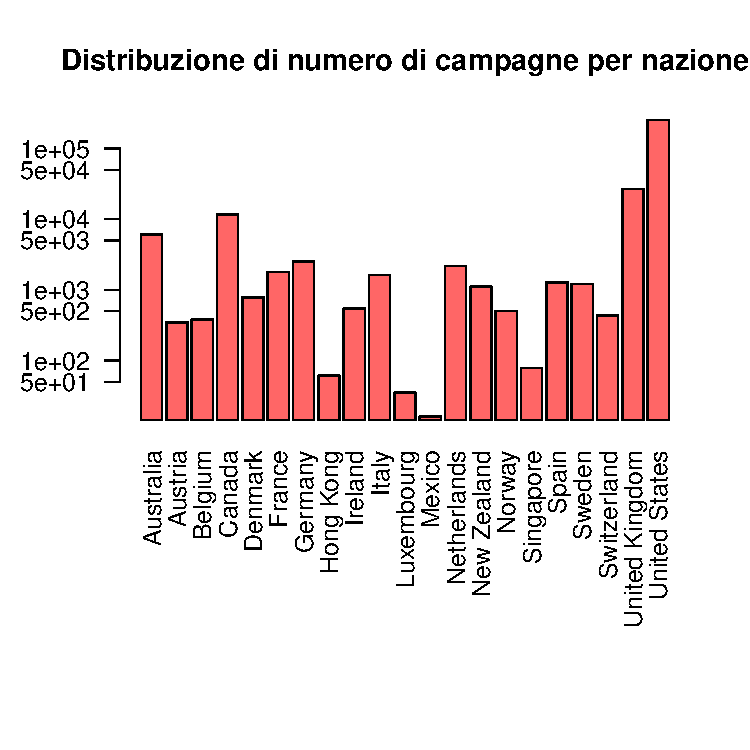
\includegraphics[width=0.45\linewidth]{../FinalResults/Images/Data_exploration_plots/barlpot_country} }}%
	\qquad
	\subfloat[Distribuzione dell'attributo rappresentante il GDP \textit{pro capite}]{{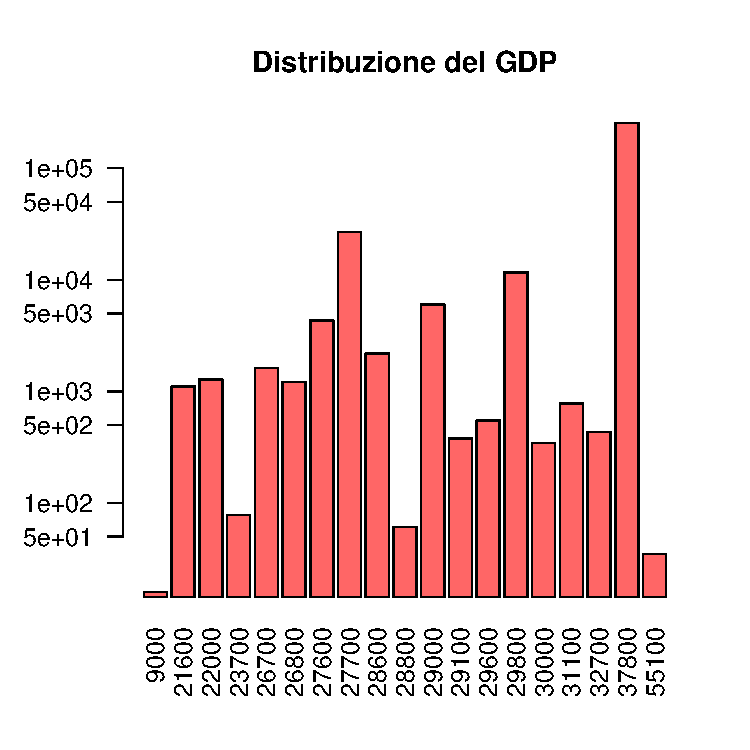
\includegraphics[width=0.45\linewidth]{../FinalResults/Images/Data_exploration_plots/barlpot_gdp}}}%
	\caption{}%
	\label{fig:countrygdp}%
\end{figure}

Sono poi stati analizzati gli attributi relativi alle categorie dei progetti proposti, quindi le feature: main category e category. 
In Figura \ref{fig:piecategory} sono riportati i grafici a torta di come si distribuiscono tra loro le 10 category più diffuse e tutte le main category.
Se la distribuzione delle 10 categorie pi diffuse è abbastanza uniforme, non vi è una categoria che domina sulle altre, altrettanto non può essere detto per le main category poiché \textit{Film \& Video}
occupa una buona percentuale seguita da \textit{Music} e \textit{Publishing}, lasciando quindi percentuali ridotte a tutte le altre categorie principali.

La distribuzione del campo service (sezione a della Figura \ref{fig:piestate}), rappresentante la percentuale di sviluppo del settore terziario nel Paese in cui è stato proposto il progetto, mostra come la maggior parte dei sample sia relativa a paesi con un settore terziario predominante sugli altri due, perché è diffuso più del 50 \%.   


Le feature goal e backer sono due attributi interi e continui che rappresentano rispettivamente la richiesta minima di denaro al fine di considerare il progetto riuscito ed il numero di donatori. Per questi due campi sono stati analizzati il valore medio e la deviazione standard; i risultati ottenuti sono stati riportati nella Tabella \ref{tab:backer}. Un valore così elevato di deviazione standard rispetto alla media, indica che i dati sono caratterizzata da una significativa varietà e distanza dal valore medio riportato.

\begin{table}[h]
	\centering
	\caption{Media e deviazione standard degli attributi goal e backers}
	\begin{tabular}{c|cc}
		Feature & Valore medio & Deviazione standard \\
		\hline  
		goal & 46672.68 & 1112774 \\ 
		backers & 102.98 & 946.76 \\ 
	\end{tabular} 
	\label{tab:backer}
\end{table}

\begin{figure}%
	\centering
	\subfloat[Distribuzione dell'attributo rappresentante la categoria specifica del progetto.]{{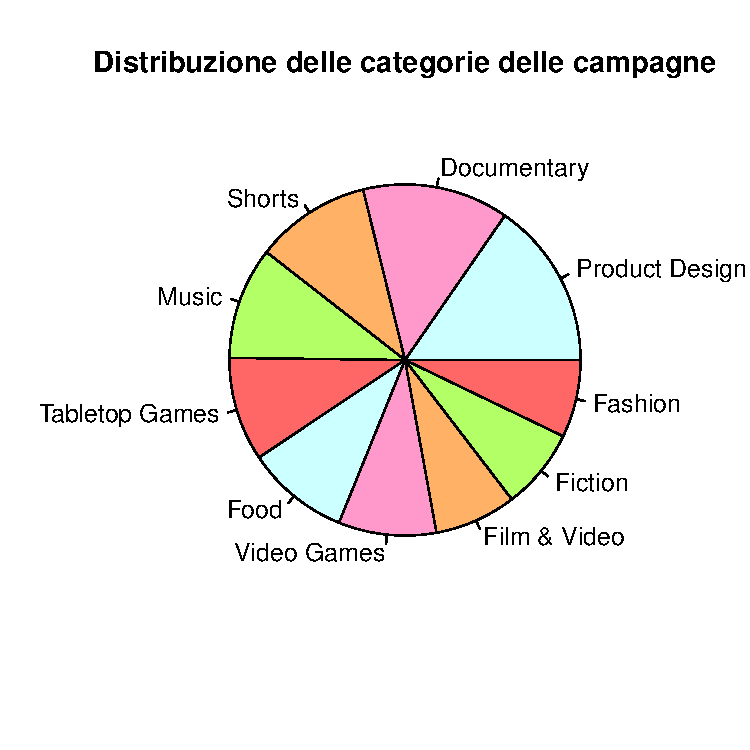
\includegraphics[width=0.45\linewidth]{../FinalResults/Images/Data_exploration_plots/pie_categories} }}%
	\qquad
	\subfloat[Distribuzione dell'attributo rappresentante la categoria generale del progetto.]{{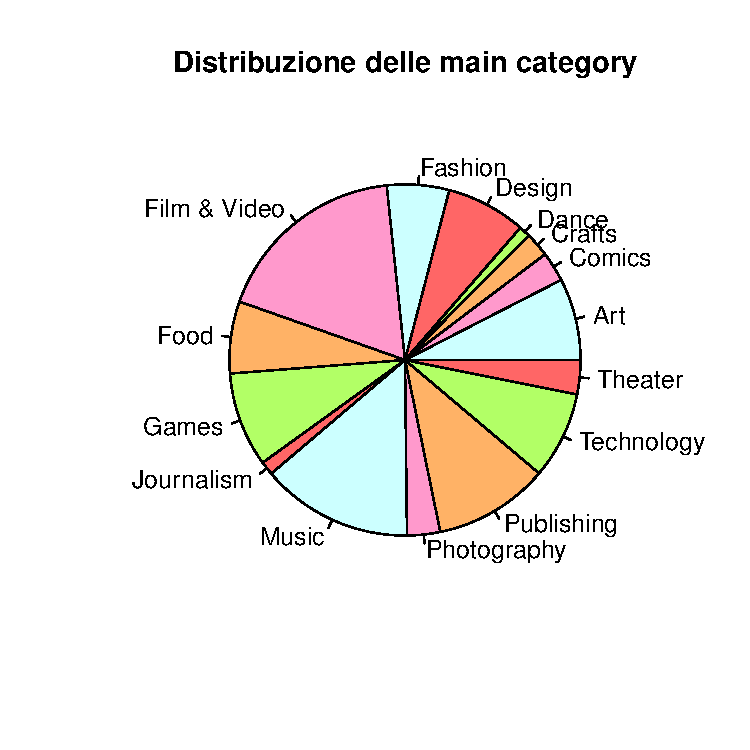
\includegraphics[width=0.45\linewidth]{../FinalResults/Images/Data_exploration_plots/pie_main_category}}}%
	\caption{}%
	\label{fig:piecategory}%
\end{figure}

L'ultimo aspetto analizzato è stata la distribuzione dell'etichettatura dei progetti, per capire come fossero divise le tuple all'interno del nostro dataset. Come mostrato nella sezione (b) della Figura \ref{fig:piestate}, la maggioranza dei sample (63 \%) in nostro possesso risultano essere relativi a progetti fallimentari. Il numero non risulta comunque tanto squilibrato da generare problemi nella fase di addestramento dei modelli di Machine Learning.

\begin{figure}%
	\centering
	\subfloat[Distribuzione dell'attributo service.]{{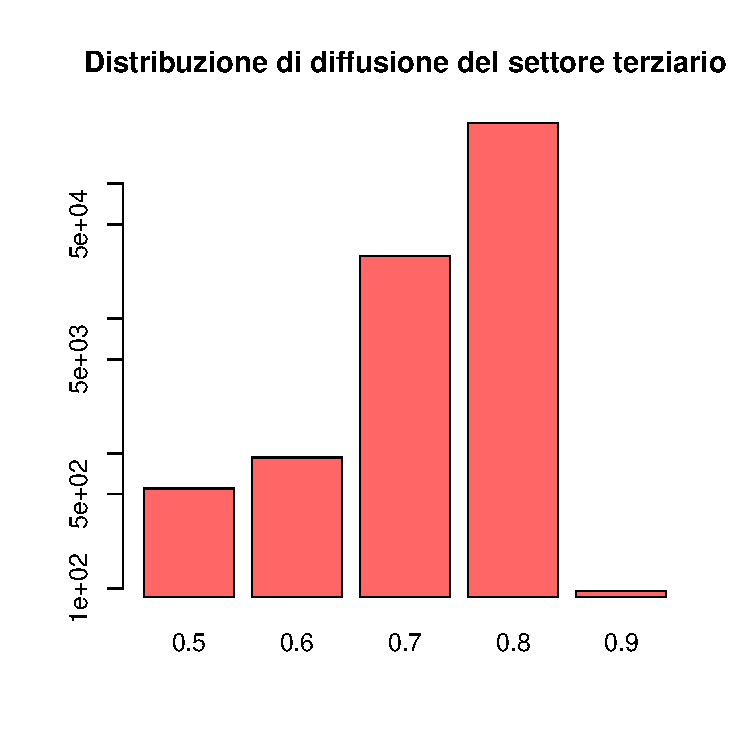
\includegraphics[width=0.4\linewidth]{../FinalResults/Images/Data_exploration_plots/barlpot_service}}}%
	\qquad
	\subfloat[Distribuzione dell'attributo state, l'etichetta dei nostri sample.]{{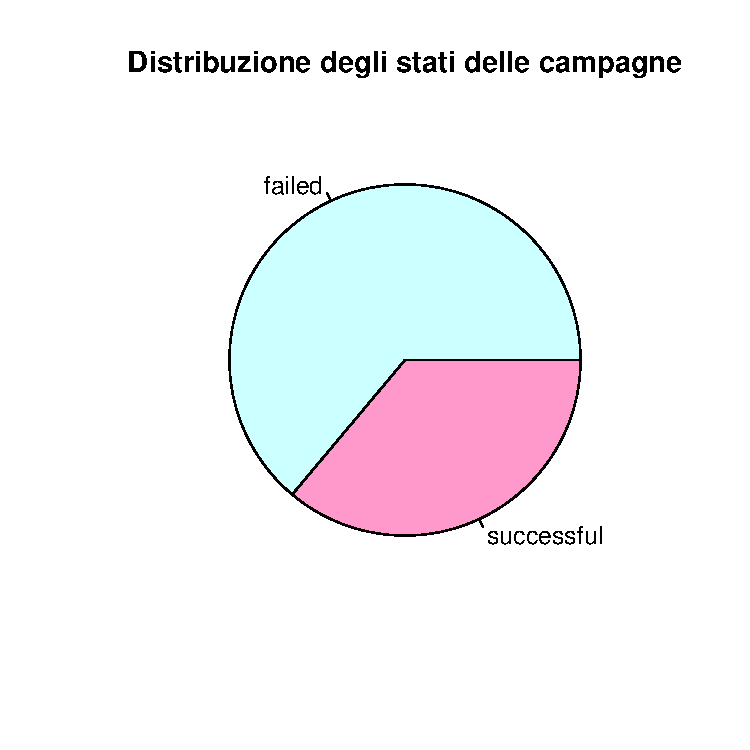
\includegraphics[width=0.4\linewidth]{../FinalResults/Images/Data_exploration_plots/pie_state}}}%
	\caption{}%
	\label{fig:piestate}%
\end{figure}

È stata infine prodotta la matrice di correlazione (mostrata in Figura \ref{fig:corrplot}) tra i vari attributi del dataset; come previsto, è emersa una evidente correlazione tra il paese in cui il progetto viene creato e i campi relativi al GDP pro capite e alla percentuale di diffusione del settore terziario nello stato. Questo poichè questi valori provengono da un dataset esterno \textit{joinato} al dataset dei progetti Kickstarter proprio sul campo nazione. Dalla matrice non emergono altre correlazioni rilevanti tra i restanti attributi del dataset.

\begin{figure}
	\centering
	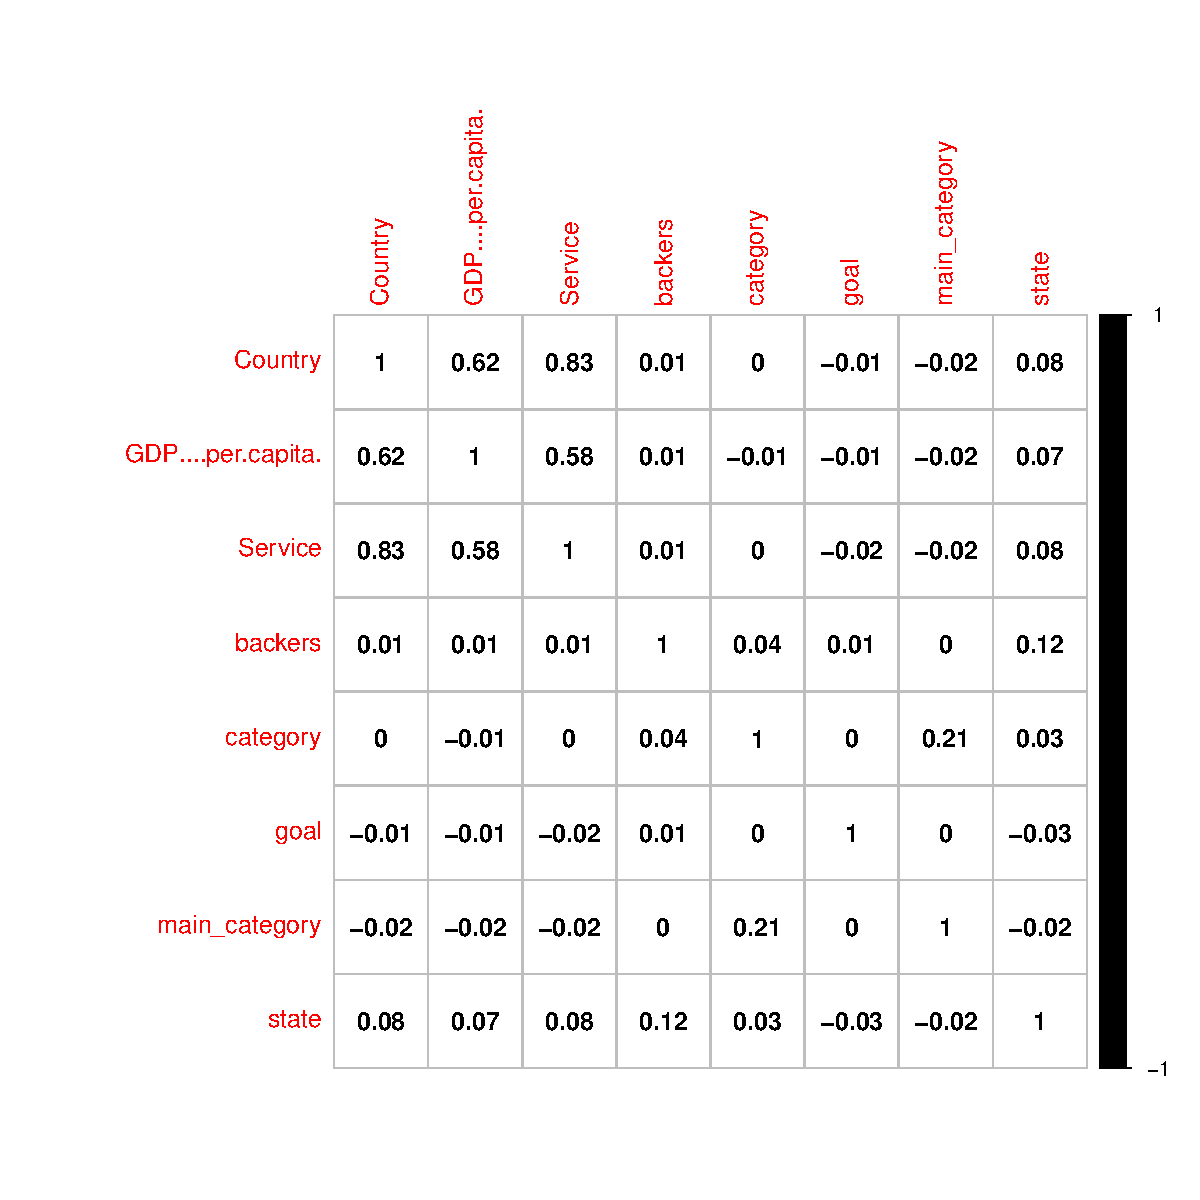
\includegraphics[width=1\linewidth]{../FinalResults/Images/Data_exploration_plots/corrplot}
	\caption{Matrice di correlazione tra le feature del dataset.}
	\label{fig:corrplot}
\end{figure}
\newpage
\section{Modelli di Machine Learning utilizzati}
In questa sezione, andremo a mostrare, dopo aver brevemente introdotto teoricamente i modelli, come tali modelli si comportano nella predizione dell'attributo state sfruttando il dataset analizzato precedentemente.
Per fare ciò, sono state utilizzate diverse misure di performance: \begin{itemize}
	\item accuratezza;
	\item precisione;
	\item recall;
	\item f-measure;
	\item la curva ROC (Receiver Operating Characteristic) e la rispettiva AUC (Area Under Curve). 
\end{itemize}
Si noti che per le misure di recall e precisione, sono stati valutati i progetti predetti correttamente come fallimentari.\\
I modelli indagati in questa relazione sono i seguenti:\begin{itemize}
	\item Baseline: fornisce una scala di riferimento per i modelli successivamente analizzati;
	\item Alberi decisionali: abbiamo deciso di analizzarli in modo da valutare quali attributi fossero ritenuti più importanti e se le decisioni potessero essere prese basandosi sul valore assunto da un sottoinsieme di tuple;
	\item Na\"ive Bayes: siamo interessati al tempo di addestramento quando utilizza dei trainset molto numerosi e con dati che non sono garantiti essere causalmente indipendenti;
	\item Support Vector Machine: vogliamo valutare il loro comportamento rispetto agli altri modelli ed approfondire l'influenza del costo rispetto al numero di vettori di supporto utilizzati per la classificazione;
	\item Reti neurali: sono al momento una delle tecniche più utilizzate in diversi ambiti, ricche di parametri che influiscono il processo di learning e classificazione.
\end{itemize}
Per i primi 3 modelli abbiamo effettuato un processo di 10-fold cross validation, in quanto i tempi di training e testing sono risultati essere contenuti; per le Support Vector Machine e le reti neurali, invece, sono stati effettuati dei processi di training utilizzando il 70 \% del dataset come insieme di istanze di training ed il restante per il testing.\\
Questa scelta è stata dettata dalle tempistiche impiegate per il training di questi modelli e dal fatto che, considerato il numero elevato di istanze presenti nel dataset (e quindi nel trainset), possiamo considerare solidi e affidabili i risultati ottenuti, poiché è improbabile che si sia presentata una suddivisione del dataset “patologica”.

\subsection{Baseline}
Al fine di avere una misura di riferimento per i modelli che saranno proposti successivamente, è stato prodotto un modello baseline, che si limita a rispondere sempre failed ad ogni sottomissione di un sample. La risposta risulta essere sempre failed in quanto, dall'analisi esplorativa dei dati effettuata in precedenza, è emerso che il valore di etichettatura più frequente era prorpio il fallimento del progetto.\\
In Figura \ref{fig:baselineperformance} e nella Tabella \ref{tab:baselineperformance} sono riportate le misure di performance ottenute con questo modello a seguito dell'operazione di 10 fold cross validation; notiamo come i valori di accuratezza e precisione si uniformino al valore di  probabilità dell'etichettatura failed nel dataset, mentre la recall rimanga ovviamente fissa ad 1.\\
Le curve ROC associate a questo modello, ripotate in Figura \ref{fig:baselineROC}, restituiscono un valore AUC molto variabile: ciò è dovuto dalla diversa distribuzione dei sample con etichettatura failed all'interno dei testset prodotti dal porcesso di 10-fold cross validation.
\begin{table}[h!]
	\caption{Tabella che riporta rispettivamente media e deviazione standard delle misure di performance in Figura \ref{fig:baselineperformance}.}
	\label{tab:baselineperformance}
	\centering
	\begin{tabular}{c|cc}
		Misura & Media & Deviazione standard \\
		\hline
		Accuracy & 0.6389 & 0.0028 \\ 
		Precision & 0.6389 & 0.0027 \\
		Recall & 1 & 0 \\
		F1Measure & 0.7797 & 0.0020 \\
	\end{tabular}
\end{table} 
\begin{figure}
	\centering
	\subfloat{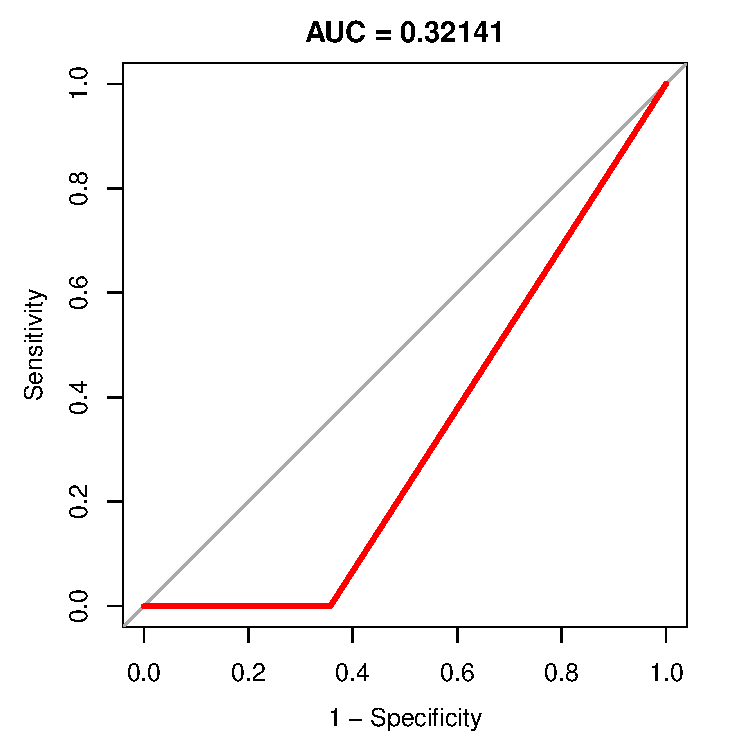
\includegraphics[width=0.3\linewidth]{../FinalResults/Images/baseline/auc_1.pdf}}\quad
	\subfloat{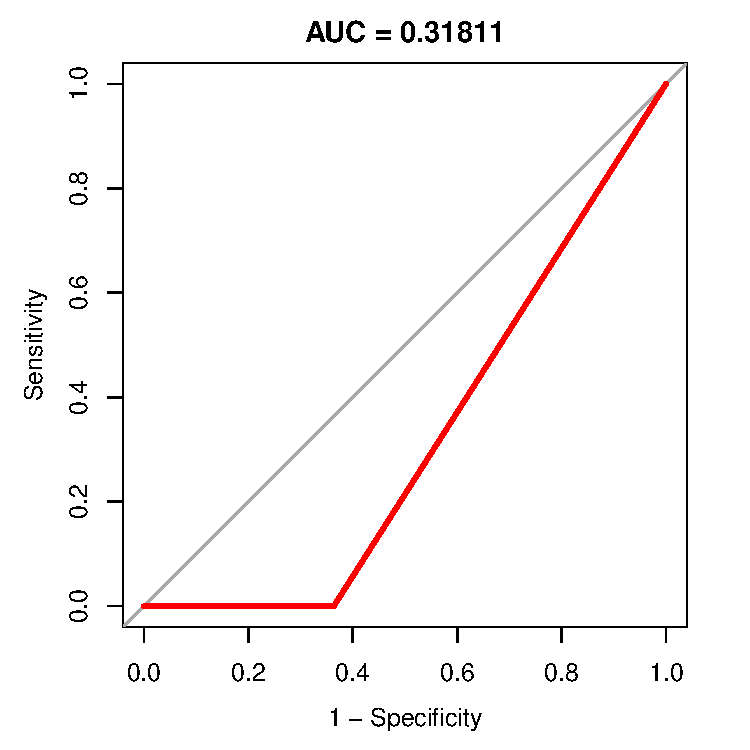
\includegraphics[width=0.3\linewidth]{../FinalResults/Images/baseline/auc_2.pdf}}\quad
	\subfloat{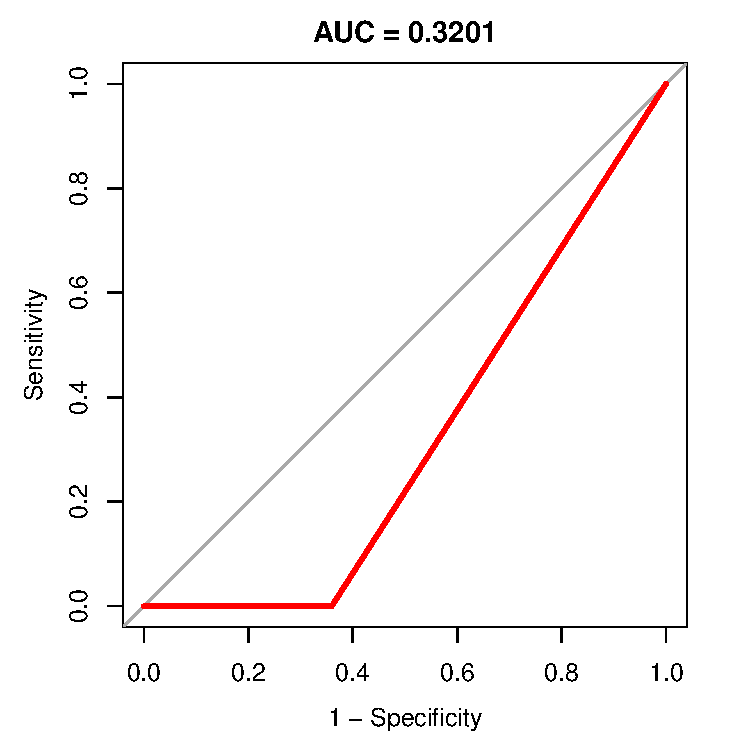
\includegraphics[width=0.3\linewidth]{../FinalResults/Images/baseline/auc_3.pdf}}\quad
	\subfloat{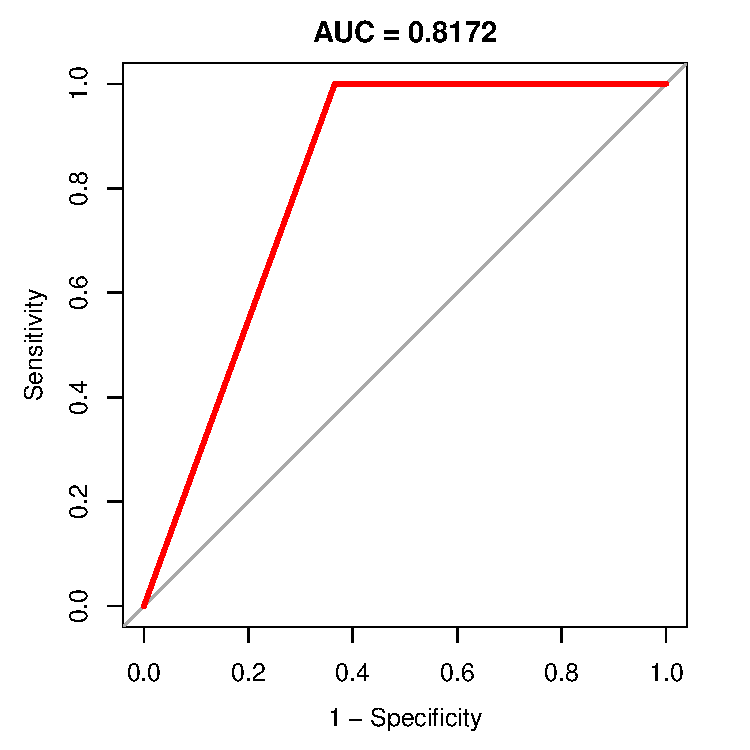
\includegraphics[width=0.3\linewidth]{../FinalResults/Images/baseline/auc_4.pdf}}\quad
	\subfloat{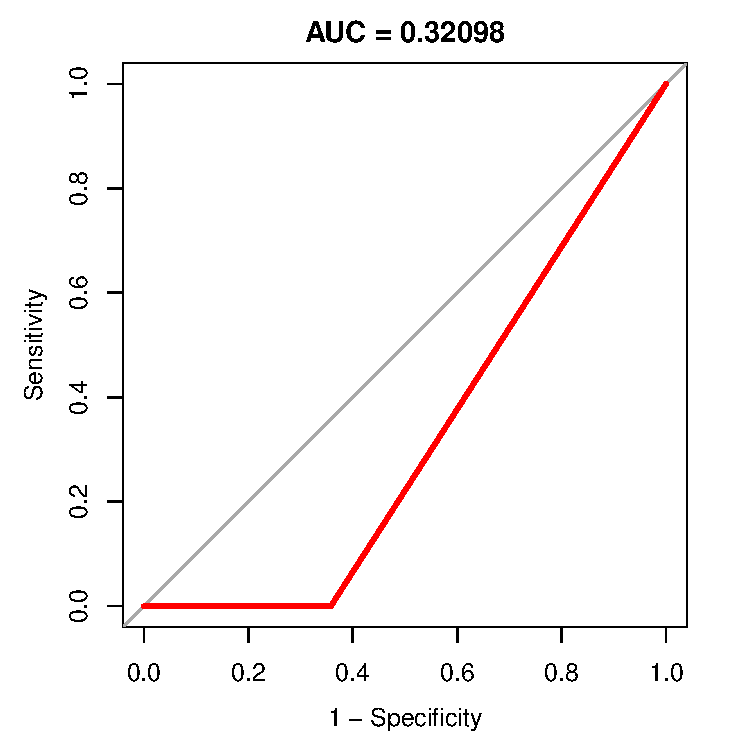
\includegraphics[width=0.3\linewidth]{../FinalResults/Images/baseline/auc_5.pdf}}\quad
	\subfloat{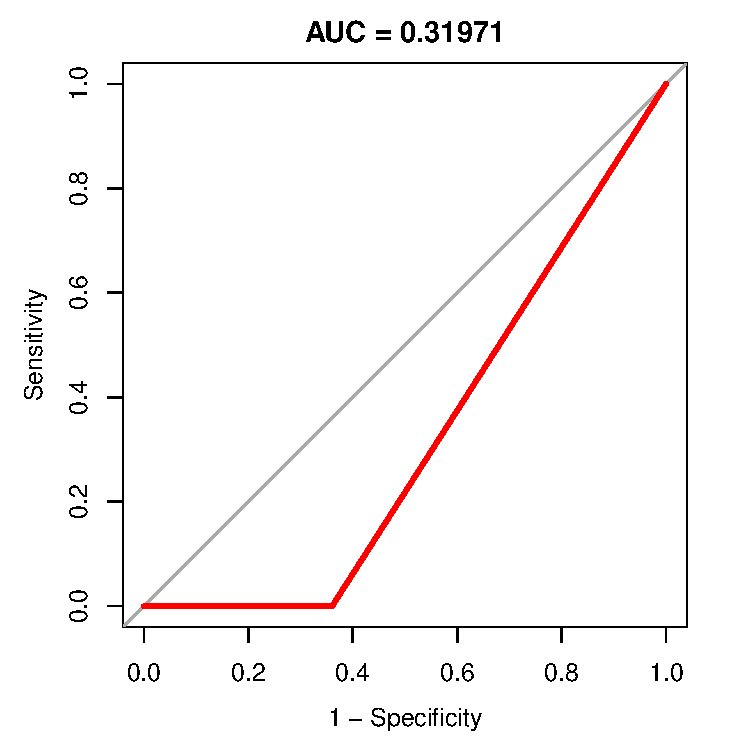
\includegraphics[width=0.3\linewidth]{../FinalResults/Images/baseline/auc_6.pdf}}\quad
	\subfloat{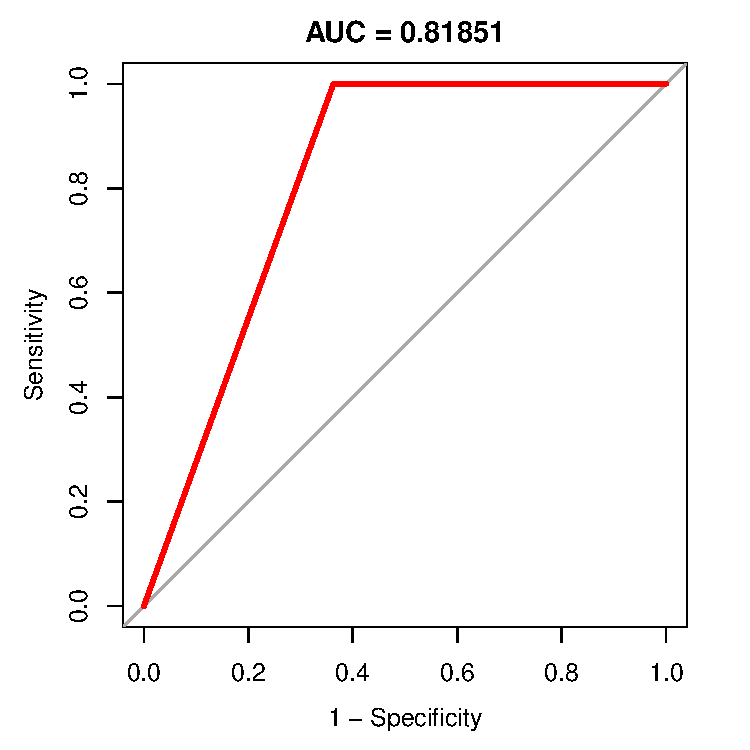
\includegraphics[width=0.3\linewidth]{../FinalResults/Images/baseline/auc_7.pdf}}\quad
	\subfloat{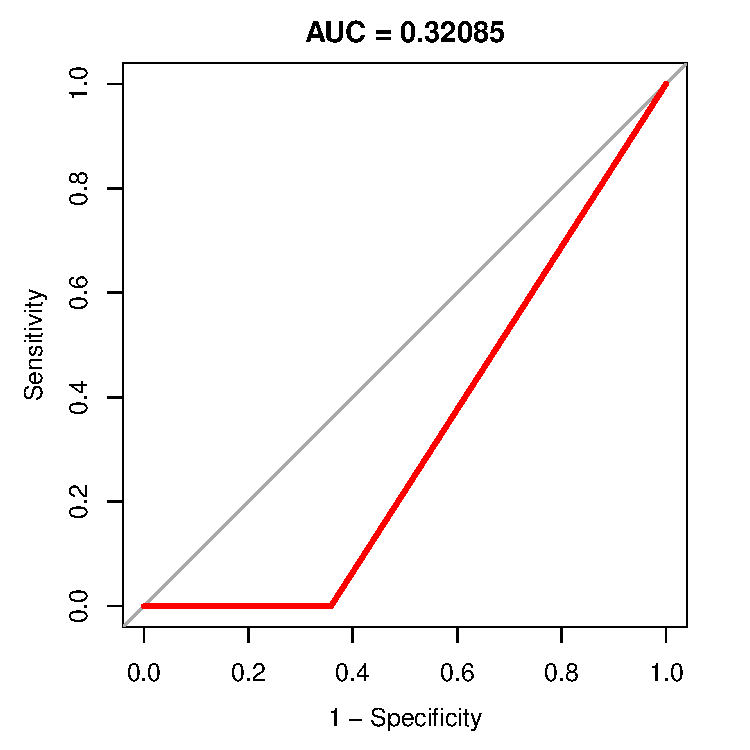
\includegraphics[width=0.3\linewidth]{../FinalResults/Images/baseline/auc_8.pdf}}\quad
	\subfloat{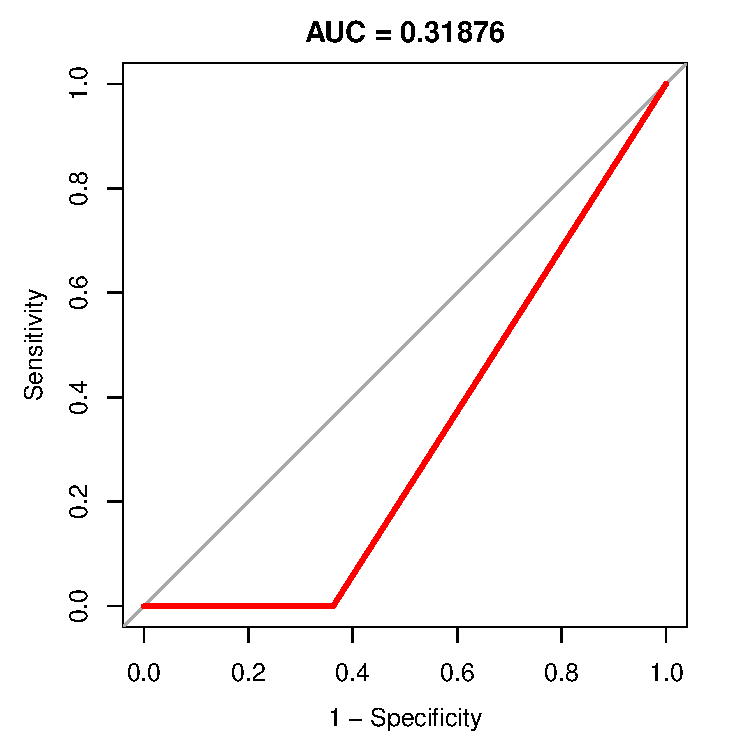
\includegraphics[width=0.3\linewidth]{../FinalResults/Images/baseline/auc_9.pdf}}\quad
	\subfloat{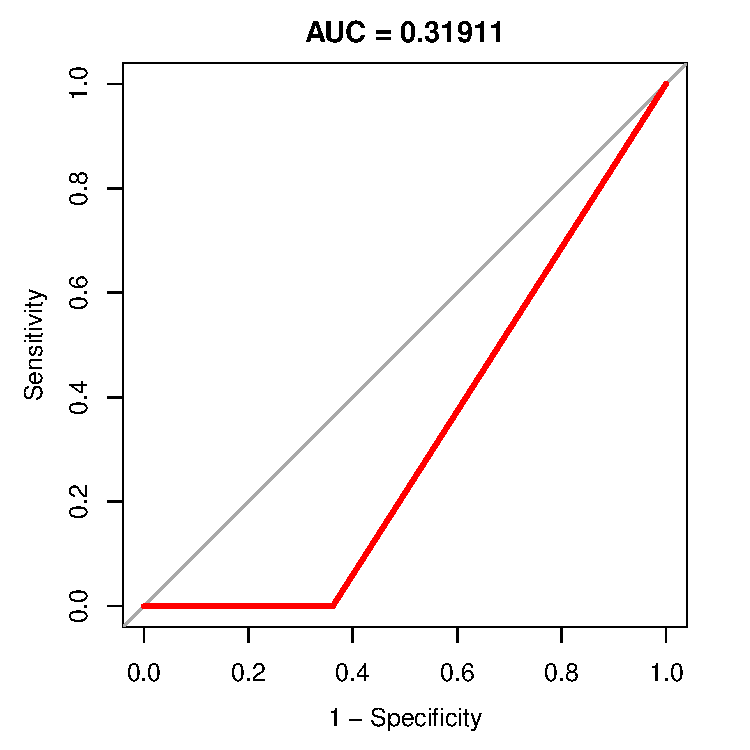
\includegraphics[width=0.3\linewidth]{../FinalResults/Images/baseline/auc_10.pdf}}\quad
	\caption{Curve ROC del modello baseline risultanti dal processo di 10-fold cross validation.}
	\label{fig:baselineROC}
\end{figure}       
\clearpage
\begin{figure}
	\centering
	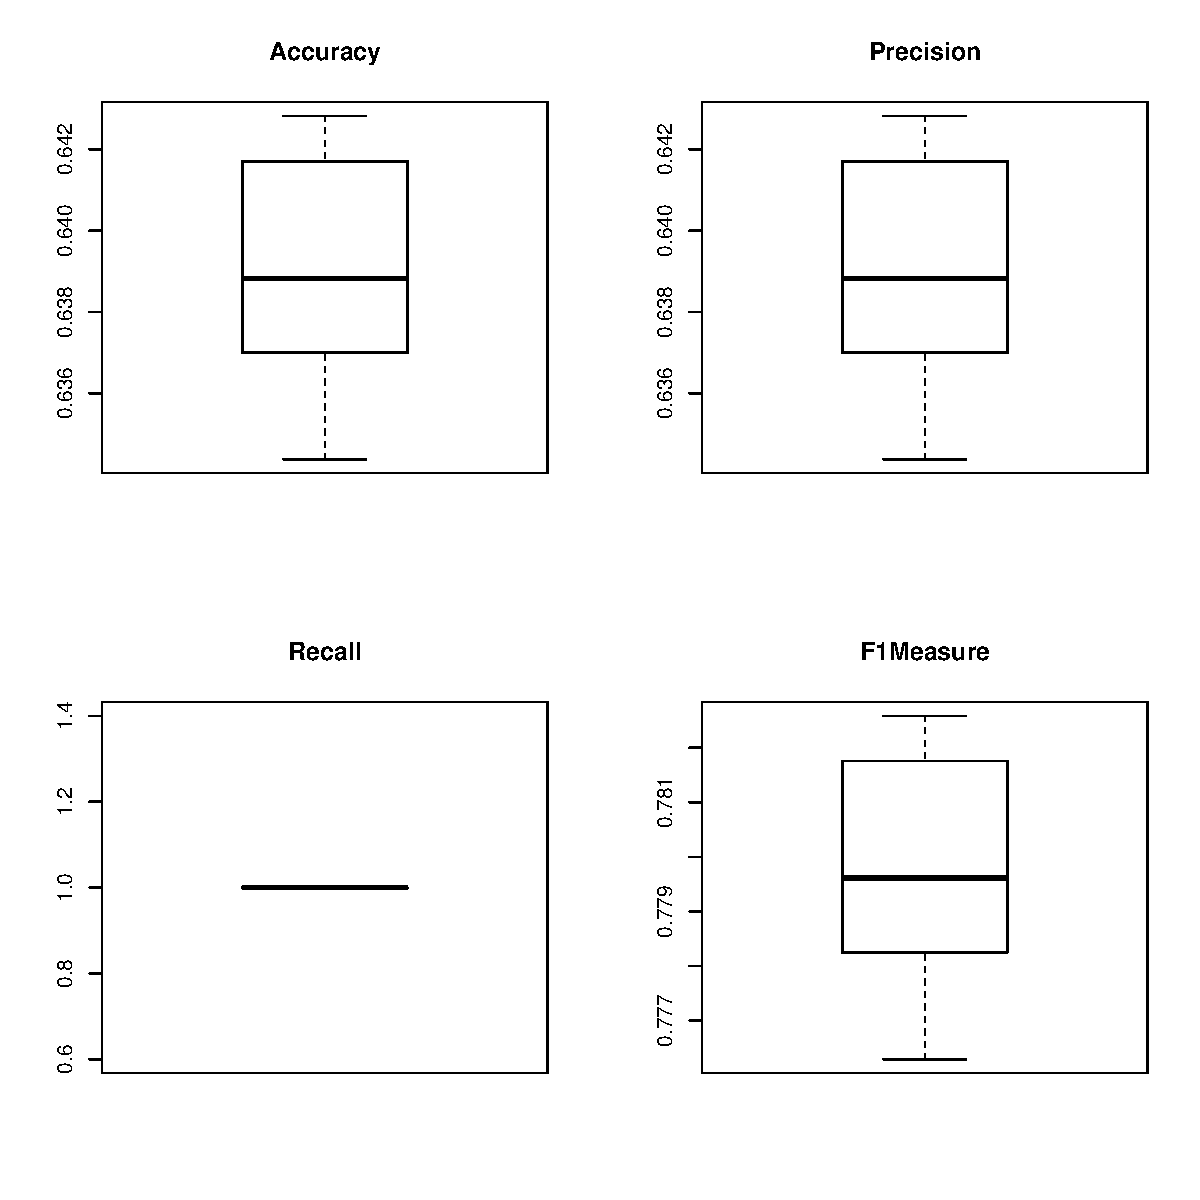
\includegraphics[width=0.7\linewidth]{../FinalResults/Baseline_performance}
	\caption{Boxplot relativi alle misure di performance del modello baseline.}
	\label{fig:baselineperformance}
\end{figure}
\subsection{Alberi decisionali}
Gli alberi decisionali sono modelli utilizzati per il Machine Learning che basano la loro tecnica di predizione su un albero etichettato, in cui ad ogni nodo viene presa la decisione del ramo in cui proseguire in base al valore dell'attributo con cui il nodo è etichettato. Le foglie di questo albero sono etichettate con il valore dell'attributo su cui si sta facendo predizione, nel nostro caso l'attributo state. La regola di decisione per le etichette segue la metrica chiamata impurità di Gini; essa è una misura della frequenza con cui un elemento scelto casualmente dall'insieme viene etichettato in modo errato se fosse etichettato in modo casuale in base alla distribuzione delle etichette nel sottoinsieme rimanente. L'impurità di Gini può essere calcolata sommando la probabilità $p_i$ di un oggetto con l'etichetta $i$ di essere scelto per la probabilità $ \sum\limits_{k\neq i} p_{k}=1-p_{i} $ di un errore nella categorizzazione di quell'elemento; questo valore raggiunge il minimo (zero) quando tutti i casi nel nodo rientrano in una singola categoria di etichettatura. .Gli alberi implementati dalla libreria \emph{R} texttt{rpart} permettono di valutare una serie di parametri, tra cui l'attributo cp, che permettono di regolare le dimensioni dell'albero prodotto e migliorarne le performance, riducendo, per quanto possibile, l'overfitting del modello.
Inizialmente è stato creato un albero che non sfruttava l'attributo backer del dataset, in quanto abbiamo immaginato che questo valore fosse di difficile stima per un utente che volesse inserire un nuovo progetto sulla piattaforma. L'albero generato si è però mostrato deludente, con performance paragonabili al modello baseline, come mostrato in Figura \ref{fig:treenbperformance} e in Tabella \ref{tab:treenbperformance}.
Le curve ROC relative a questo modello (riportate in Figura \ref{fig:treeNBROC}) sono risultate essere molto simili nelle varie iterazioni, mostrando un maggiore livello di solidità circa la composizione del trainset e del testset rispetto al modello baseline.
\begin{table}[h!]
	\caption{Tabella che riporta rispettivamente media e deviazione standard delle misure in Figura \ref{fig:treenbperformance}.}
	\label{tab:treenbperformance}
	\centering
	\begin{tabular}{c|cc}
		Misura & Media & Deviazione standard \\
		\hline
		Accuracy & 0.6814 & 0.0019 \\ 
		Precision & 0.7084 & 0.0036 \\
		Recall & 0.8521 & 0.0084 \\
		F1Measure & 0.7736 & 0.0024 \\
	\end{tabular}
\end{table}
\begin{figure}[h!]
	\centering
	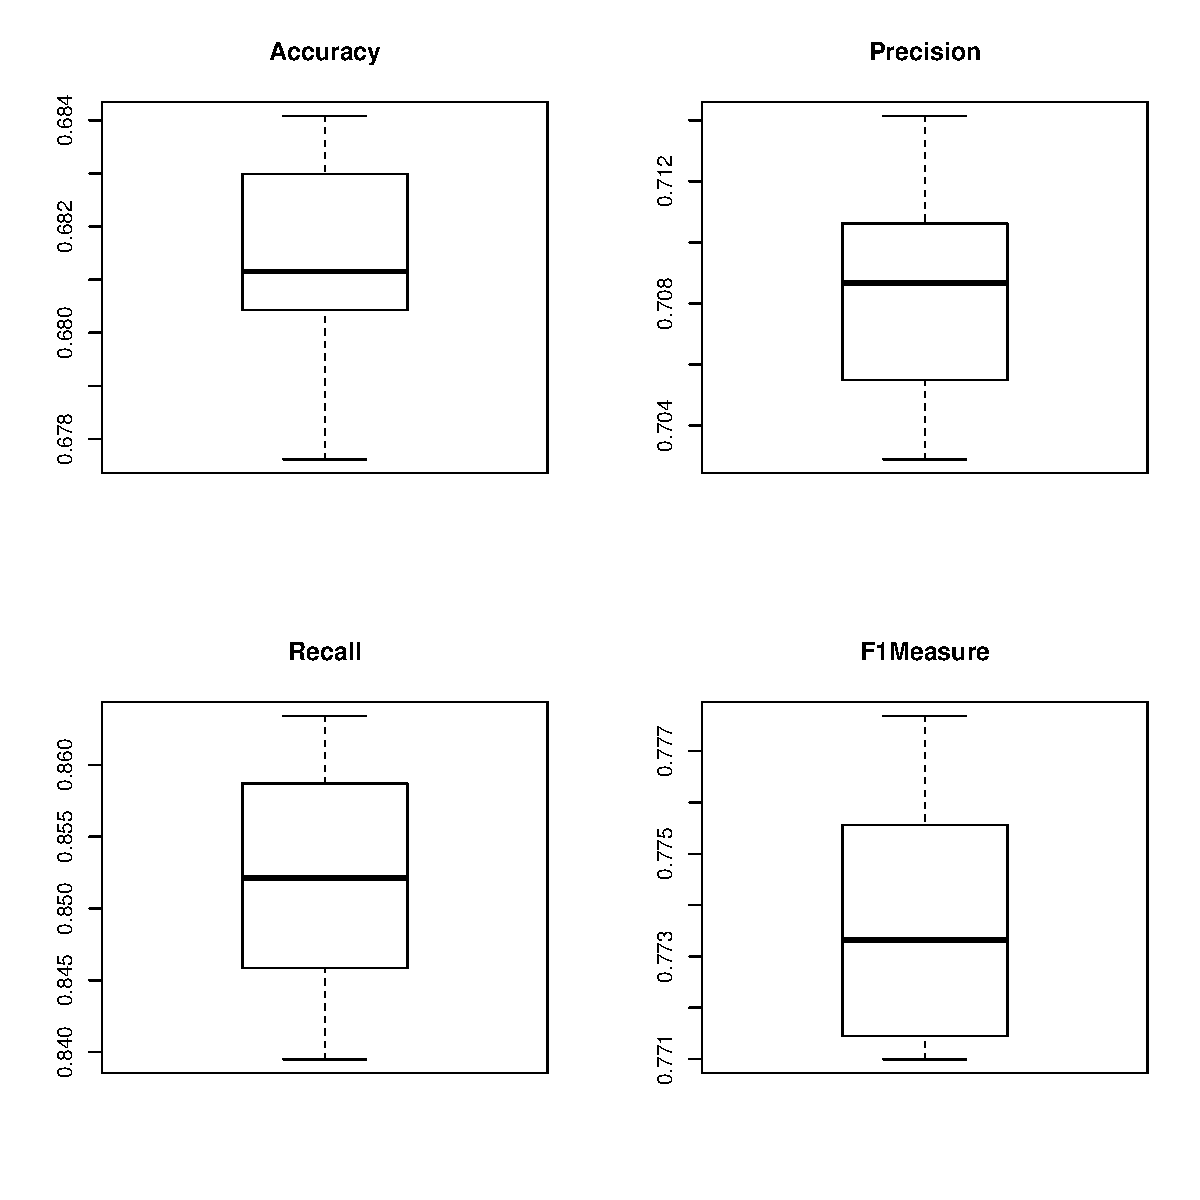
\includegraphics[width=0.7\linewidth]{../FinalResults/TreeNB_performance}
	\caption{Boxplot relativi alle misure di performance dell'albero di decisione senza l'utilizzo della feature backer.}
	\label{fig:treenbperformance}
\end{figure}
\begin{figure}[h!]
	\centering
	\subfloat{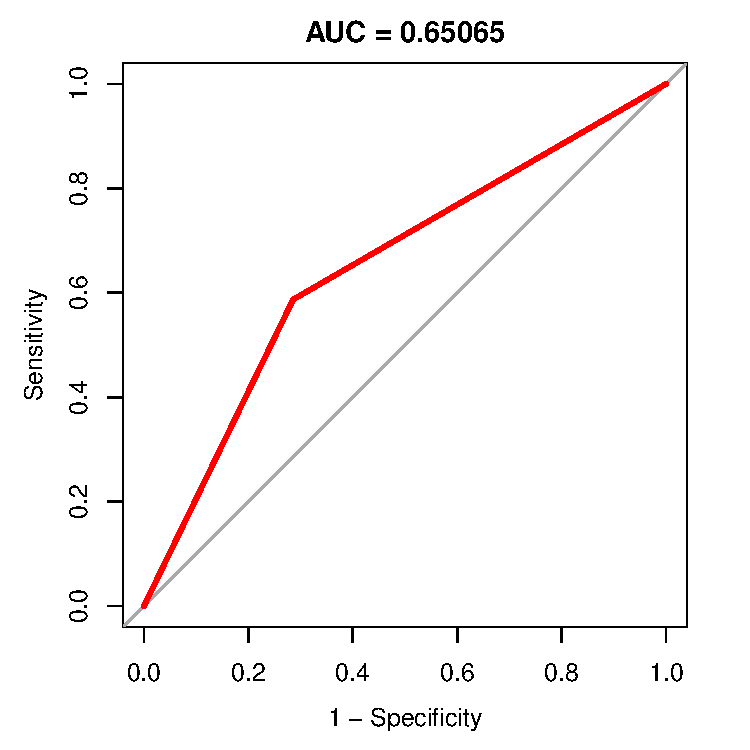
\includegraphics[width=0.3\linewidth]{../FinalResults/Images/treeNB/auc_1.pdf}}\quad
	\subfloat{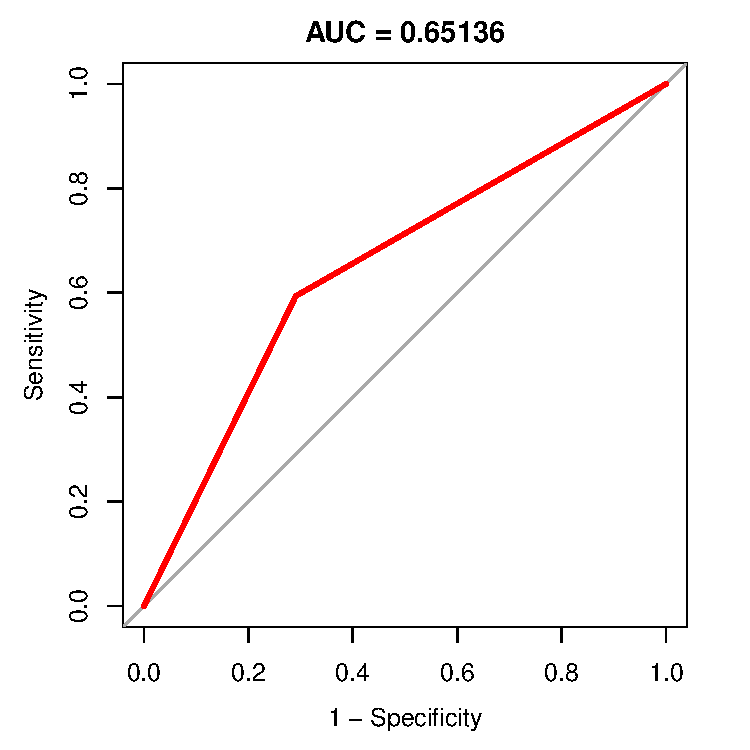
\includegraphics[width=0.3\linewidth]{../FinalResults/Images/treeNB/auc_2.pdf}}\quad
	\subfloat{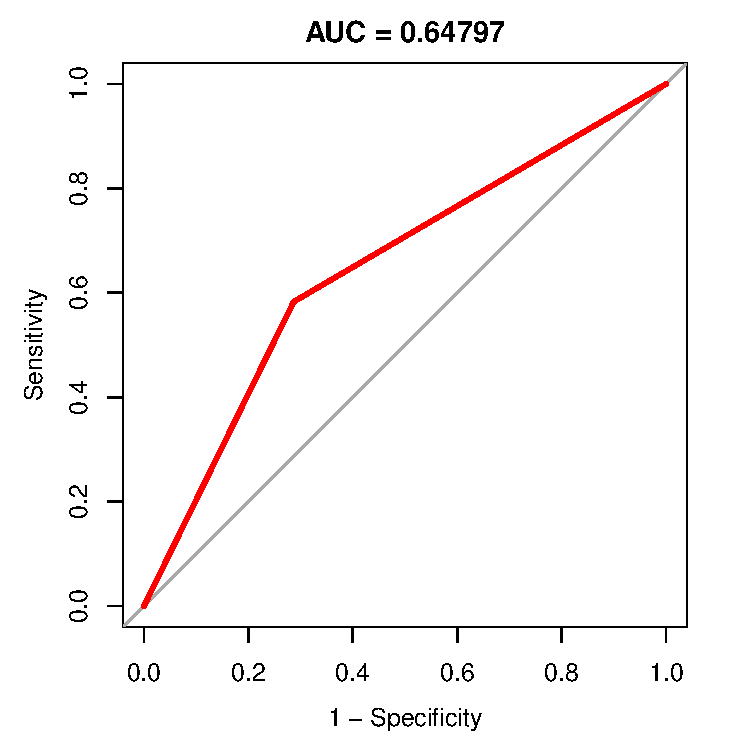
\includegraphics[width=0.3\linewidth]{../FinalResults/Images/treeNB/auc_3.pdf}}\quad
	\subfloat{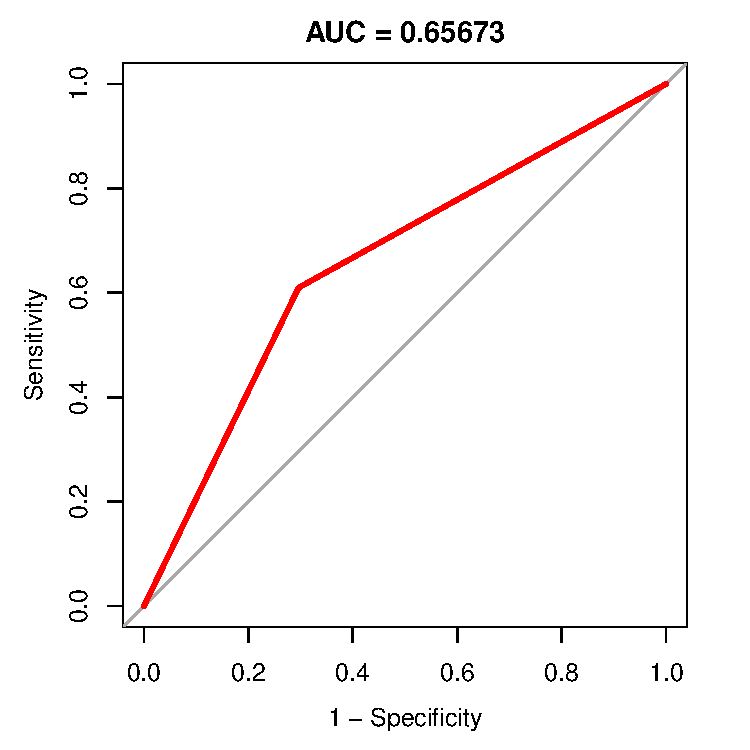
\includegraphics[width=0.3\linewidth]{../FinalResults/Images/treeNB/auc_4.pdf}}\quad
	\subfloat{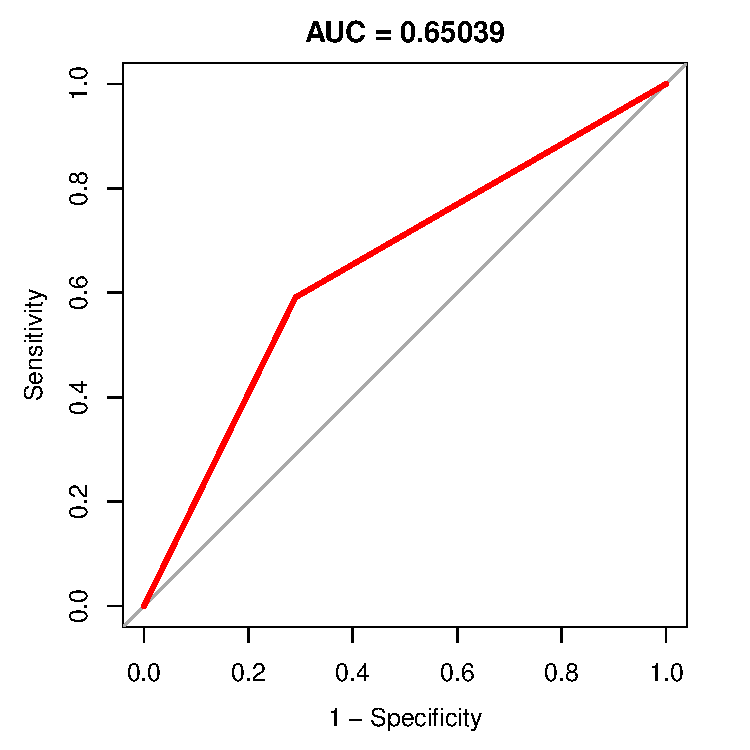
\includegraphics[width=0.3\linewidth]{../FinalResults/Images/treeNB/auc_5.pdf}}\quad
	\subfloat{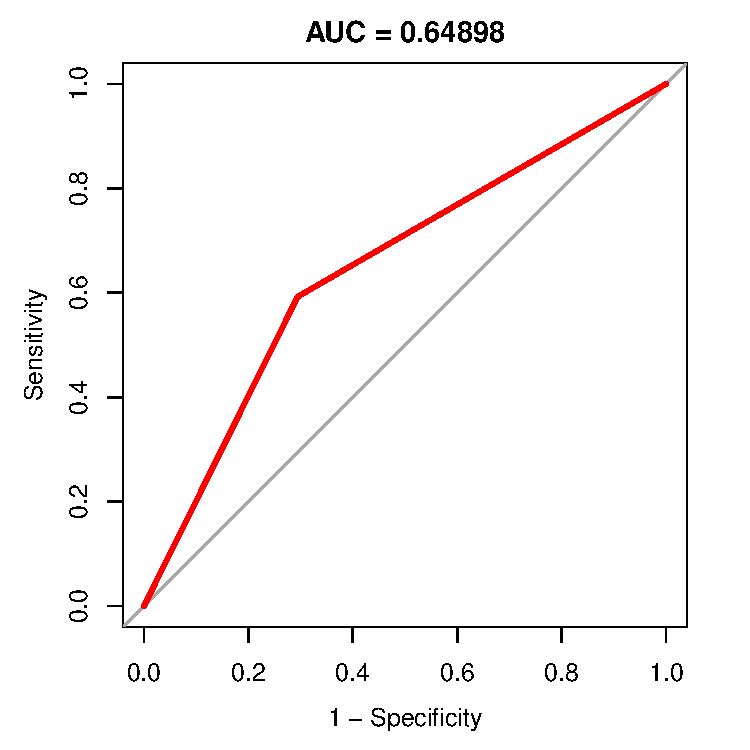
\includegraphics[width=0.3\linewidth]{../FinalResults/Images/treeNB/auc_6.pdf}}\quad
	\subfloat{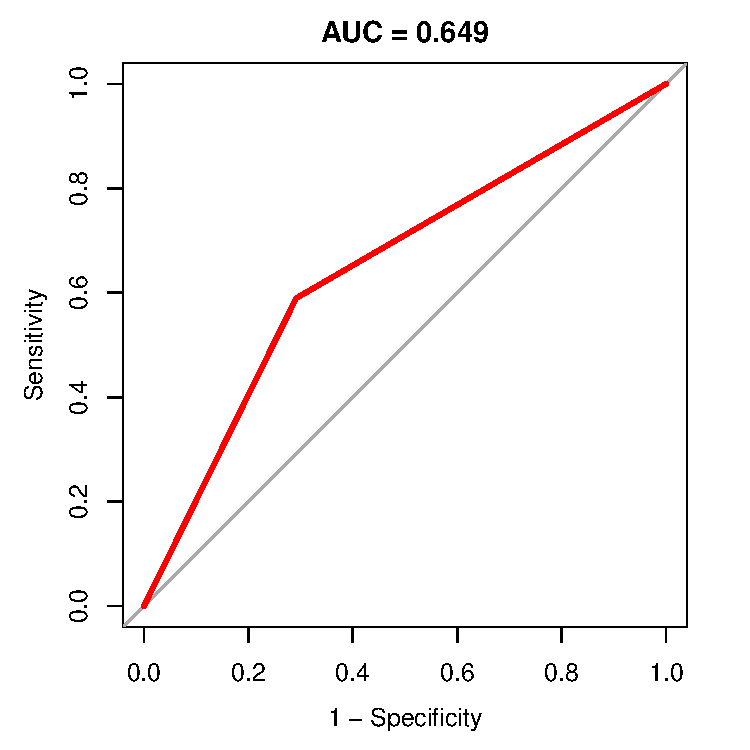
\includegraphics[width=0.3\linewidth]{../FinalResults/Images/treeNB/auc_7.pdf}}\quad
	\subfloat{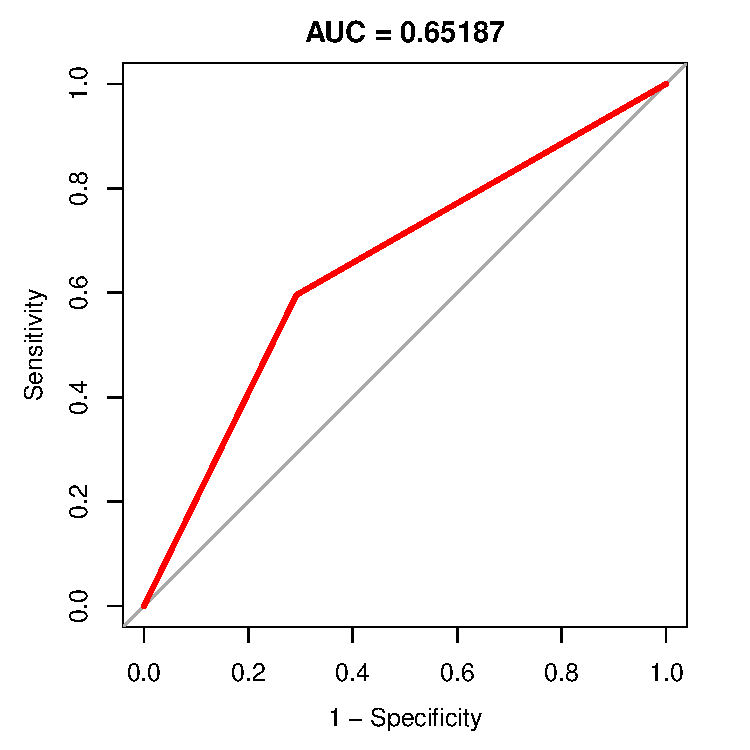
\includegraphics[width=0.3\linewidth]{../FinalResults/Images/treeNB/auc_8.pdf}}\quad
	\subfloat{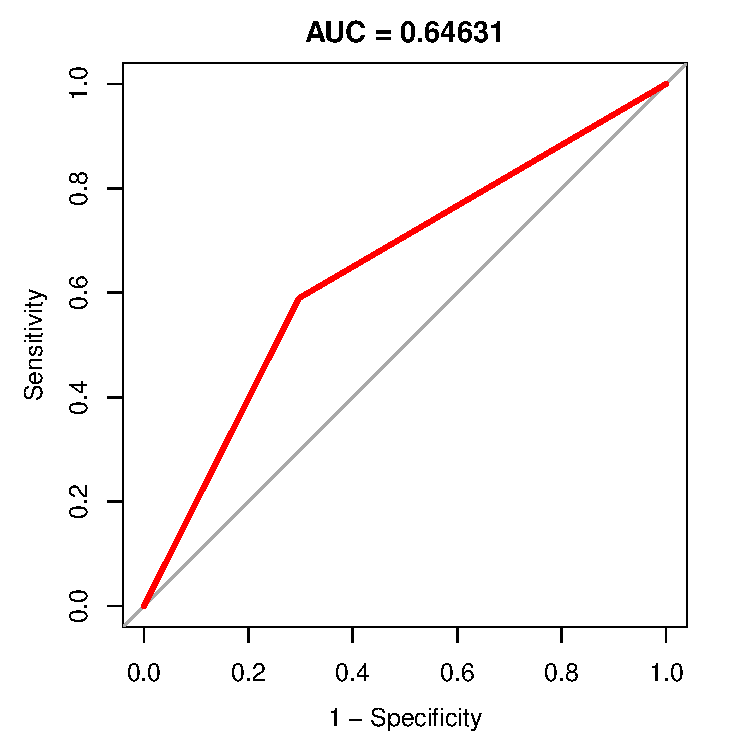
\includegraphics[width=0.3\linewidth]{../FinalResults/Images/treeNB/auc_9.pdf}}\quad
	\subfloat{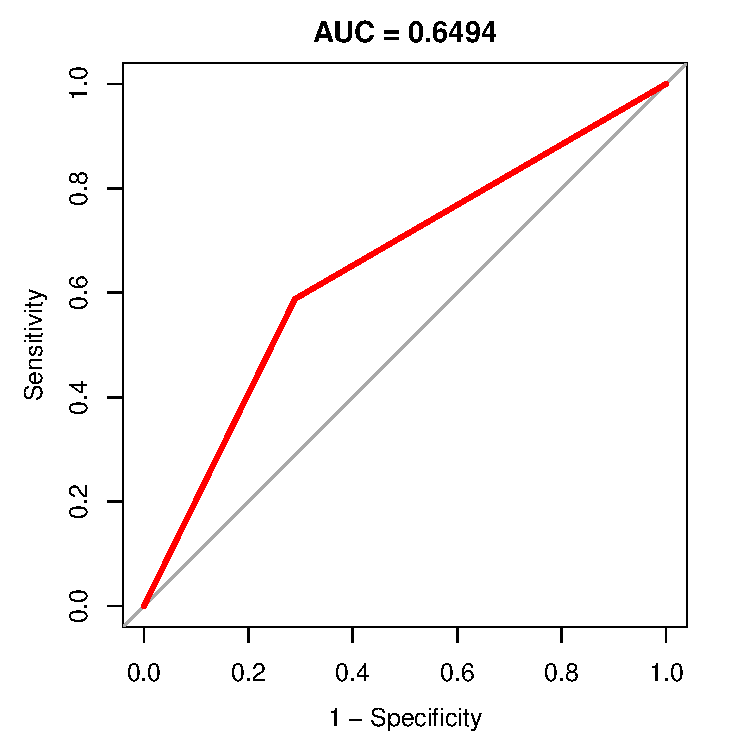
\includegraphics[width=0.3\linewidth]{../FinalResults/Images/treeNB/auc_10.pdf}}\quad
	\caption{Curve ROC del modello ad albero senza l'utilizzo della feature baker risultanti dal processo di 10-fold cross validation.}
	\label{fig:treeNBROC}
\end{figure}  
\newpage
È stato quindi deciso di sfruttare tutte le feature disponibili, supponendo che per futuri progetti non ancora realizzati sarà possibile stimare il valore dei backer tramite l'utilizzo di modelli di regressione lineare. L'albero prodotto dal processo di addestramento è mostrato in Figura \ref{fig:tree}. Le performance ottenute dal nuovo modello sono decisamente superiori al precedente, come mostrato nella Tabella \ref{tab:treeperformance} e in Figura \ref{fig:treeperformance}.\\
\begin{figure}
	\centering
	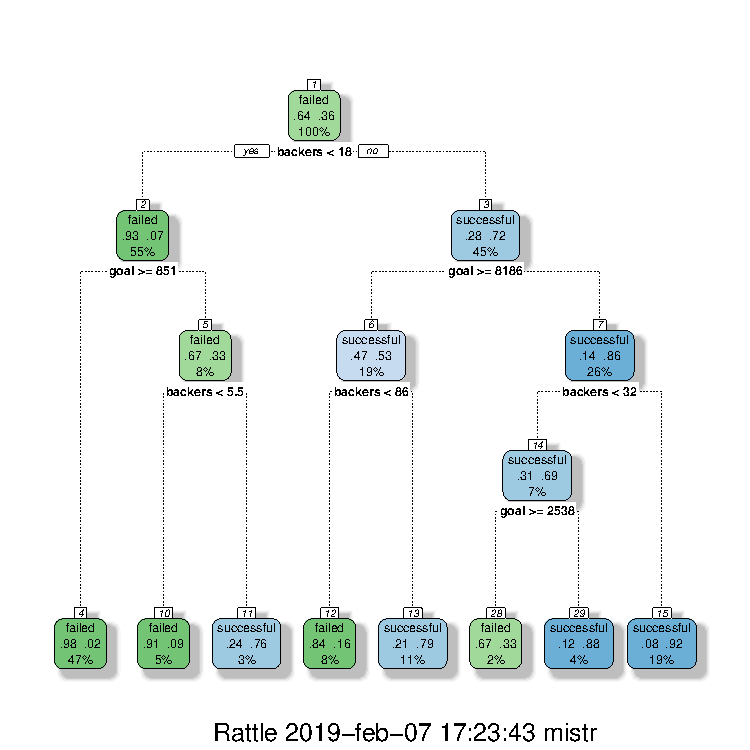
\includegraphics[width=0.9\linewidth]{../FinalResults/tree}
	\caption{Albero prodotto dal processo di addestramento con tutte le feature del dataset.}
	\label{fig:tree}
\end{figure}
Le feature utilizzate dal modello sono esclusivamente il numero di backer e il goal del progetto, gli altri campi del dataset non sono utilizzati per la classificazione. Ciononostante le performance ottenute da questo modello si sono rivelate più che discrete, superando nettamente il modello baseline proposto. La scarsissima varianza dei valori durante il processo di 10-fold cross validation mostra come il modello prodotto sia solido e non sensibile a eventuali eterogeneità di distribuzione di tuple etichettate come fallite o riuscite. Questo si ripercuote anche sulle curve ROC, riportate in Figura \ref{fig:treeROC}, il cui andamento è pressoché identico durante tutte le 10 iterazioni di validazione.

\begin{table}[h!]
	\caption{Tabella che riporta rispettivamente media e deviazione standard delle misure in Figura \ref{fig:treeperformance}.}
	\label{tab:treeperformance}
	\centering
	\begin{tabular}{c|cc}
		Misura & Media & Deviazione standard \\
		\hline
		Accuracy & 0.9112 & 0.0021 \\ 
		Precision & 0.9376 & 0.0030 \\
		Recall & 0.9224 & 0.0019 \\
		F1Measure & 0.9299 & 0.0018 \\
	\end{tabular}
\end{table}
\begin{figure}[h!]
	\centering
	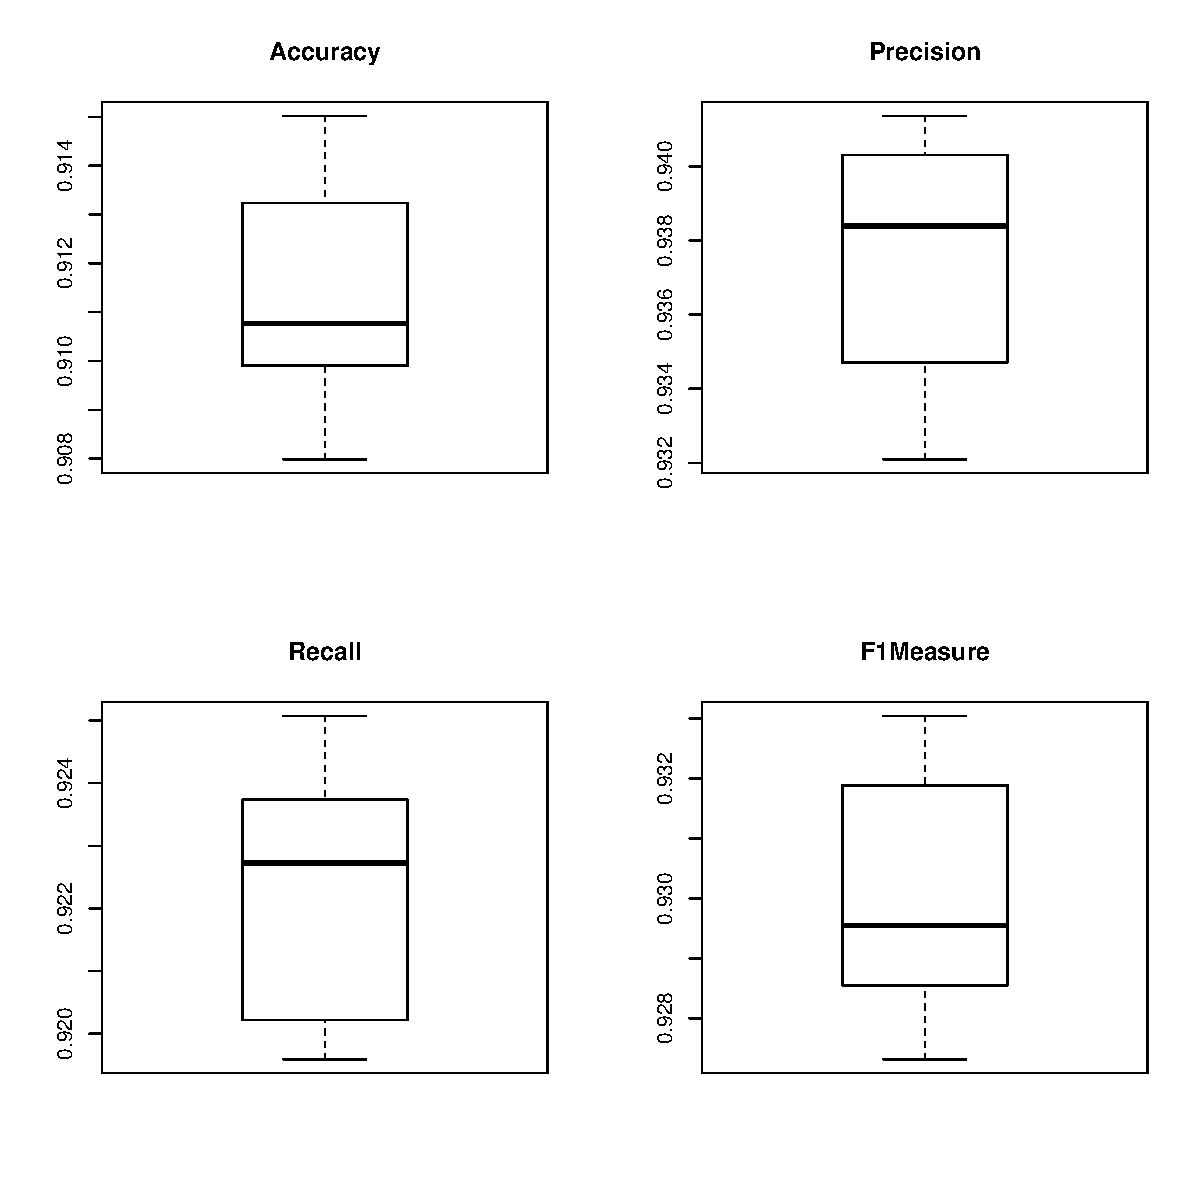
\includegraphics[width=0.7\linewidth]{../FinalResults/Tree_performance}
	\caption{Boxplot relativi alle misure di performance dell'albero di decisione con tutte le feature.}
	\label{fig:treeperformance}
\end{figure}
\begin{figure}[h!]
	\centering
	\subfloat{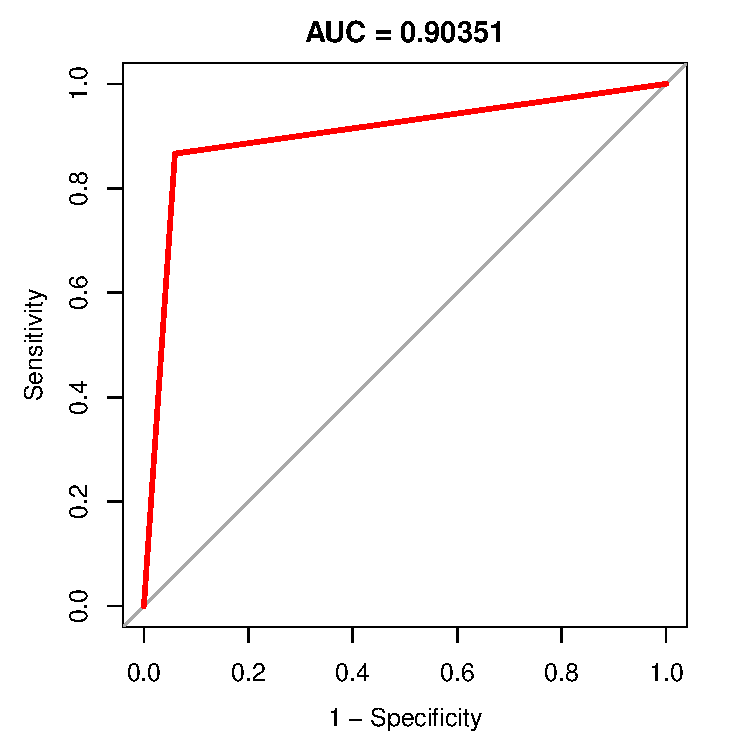
\includegraphics[width=0.3\linewidth]{../FinalResults/Images/tree/auc_1.pdf}}\quad
	\subfloat{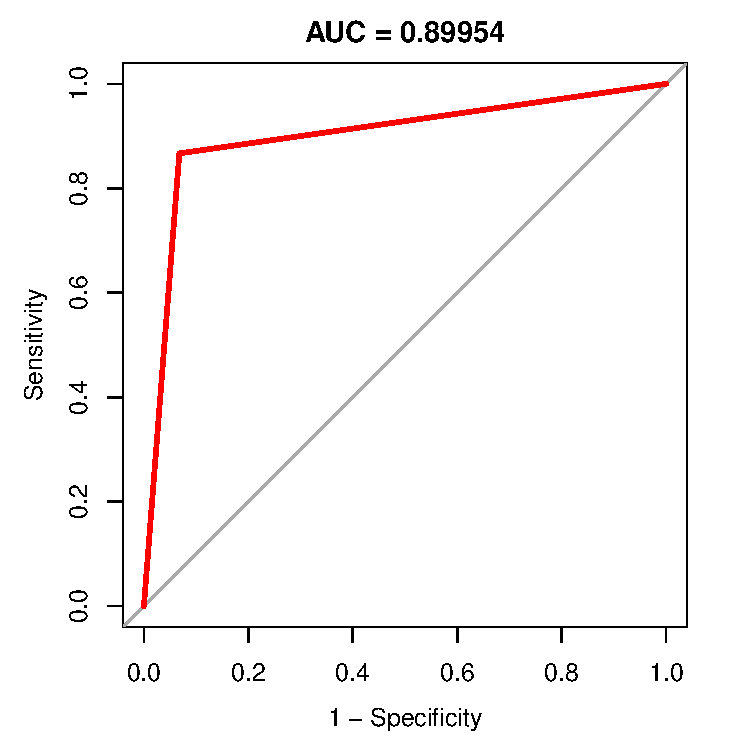
\includegraphics[width=0.3\linewidth]{../FinalResults/Images/tree/auc_2.pdf}}\quad
	\subfloat{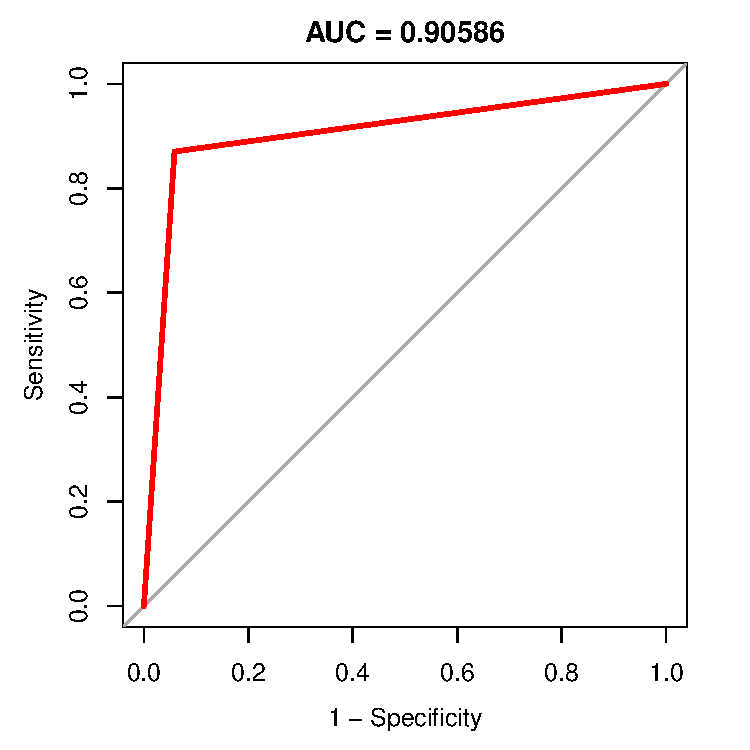
\includegraphics[width=0.3\linewidth]{../FinalResults/Images/tree/auc_3.pdf}}\quad
	\subfloat{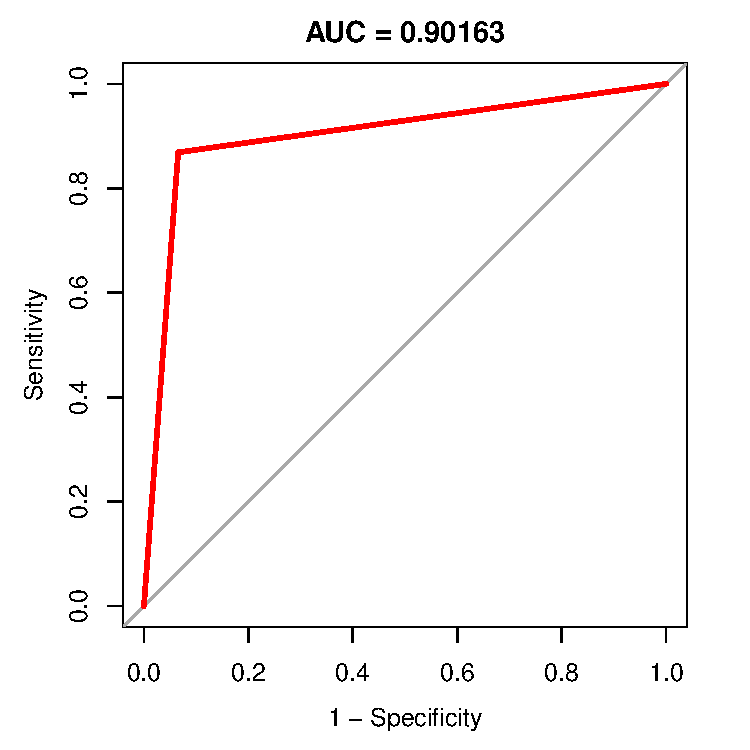
\includegraphics[width=0.3\linewidth]{../FinalResults/Images/tree/auc_4.pdf}}\quad
	\subfloat{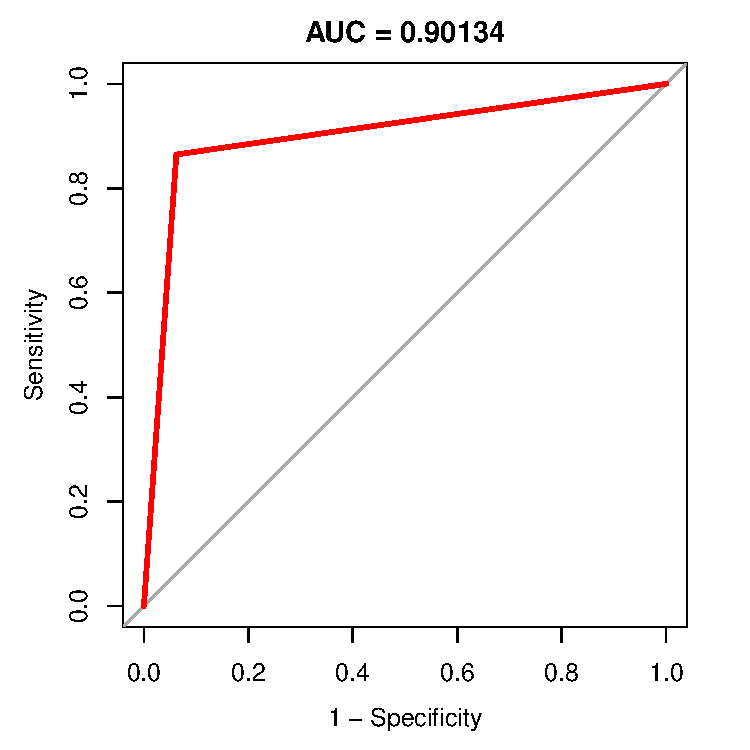
\includegraphics[width=0.3\linewidth]{../FinalResults/Images/tree/auc_5.pdf}}\quad
	\subfloat{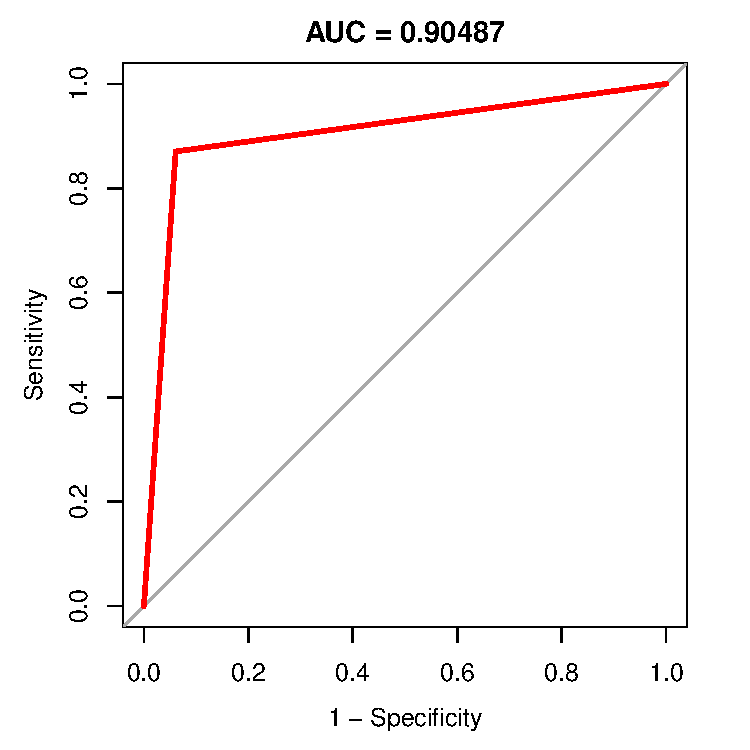
\includegraphics[width=0.3\linewidth]{../FinalResults/Images/tree/auc_6.pdf}}\quad
	\subfloat{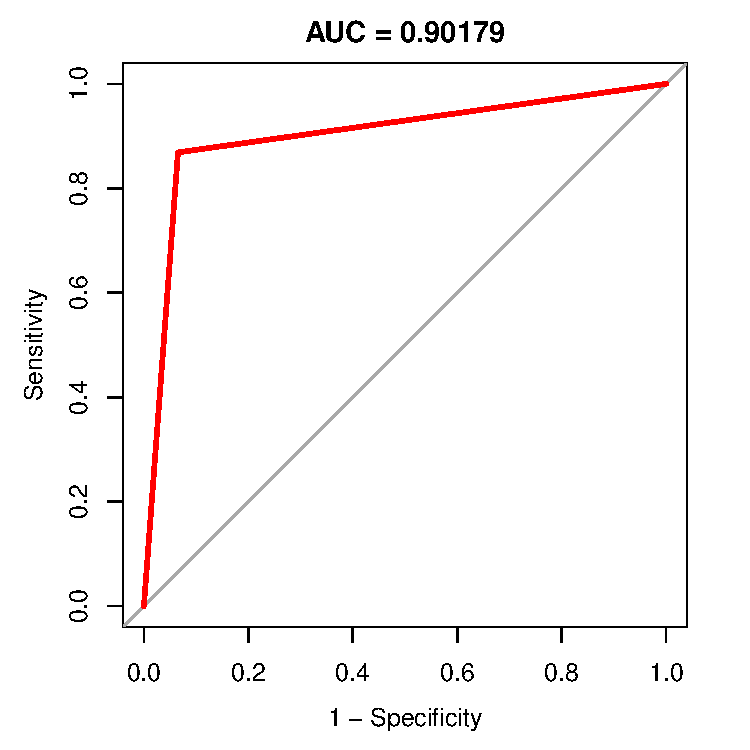
\includegraphics[width=0.3\linewidth]{../FinalResults/Images/tree/auc_7.pdf}}\quad
	\subfloat{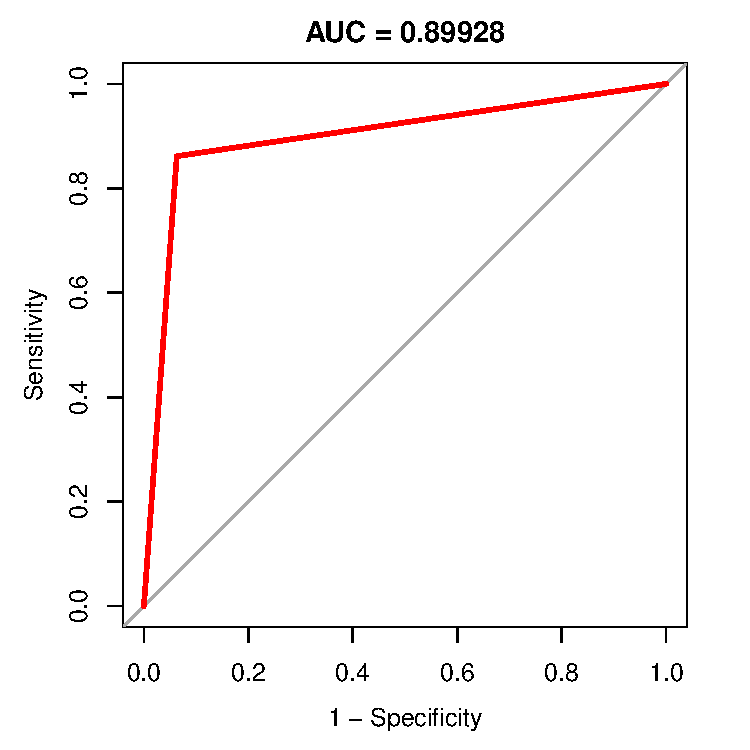
\includegraphics[width=0.3\linewidth]{../FinalResults/Images/tree/auc_8.pdf}}\quad
	\subfloat{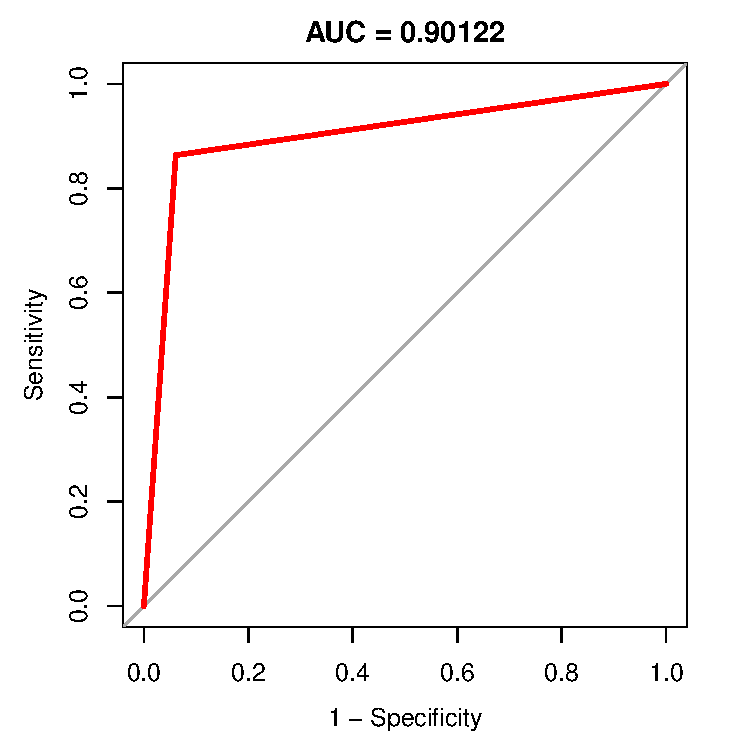
\includegraphics[width=0.3\linewidth]{../FinalResults/Images/tree/auc_9.pdf}}\quad
	\subfloat{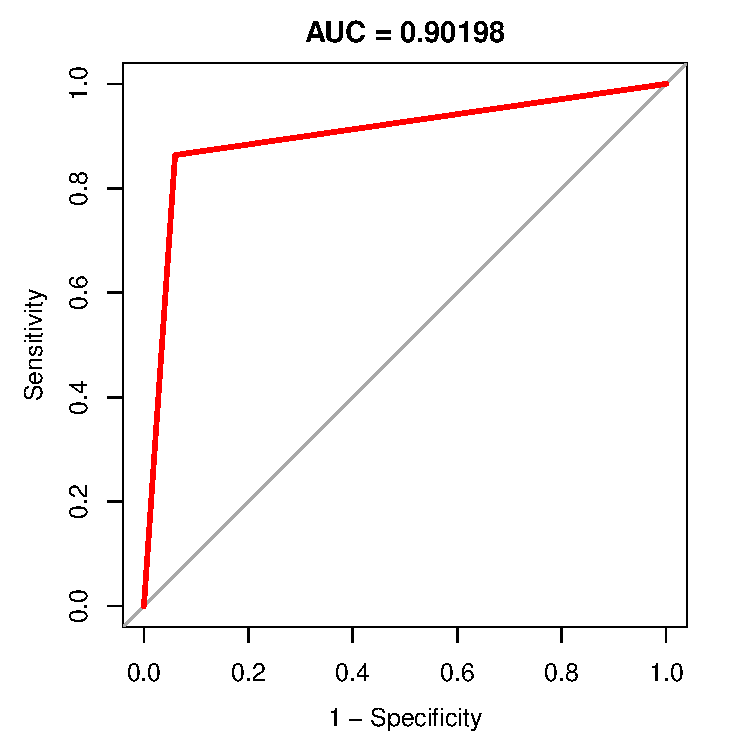
\includegraphics[width=0.3\linewidth]{../FinalResults/Images/tree/auc_10.pdf}}\quad
	\caption{Curve ROC del modello ad albero risultanti dal processo di 10-fold cross validation.}
	\label{fig:treeROC}
\end{figure}   

Infine, abbiamo valutato il parametro di complessità dell'albero prodotto. Il grafico (riportato in Figura \ref{fig:cptree}), seppur mostrando un valore di complessità molto basso, mostra come sia effettivamente possibile effettuare una potatura di alcuni rami pagando un costo in performance predittive infinitesimale. Abbiamo quindi deciso di effettuare la potatura dell'albero ponendo il valore del parametro cp a $0.015$, ottenendo così l'albero riportato in Figura \ref{fig:prunedtree}. Le misure di performance, non riportate di seguito per questioni di brevità, sono completamente assimilabili a quelle riportate per l'albero non potato.
\begin{figure}
	\centering
	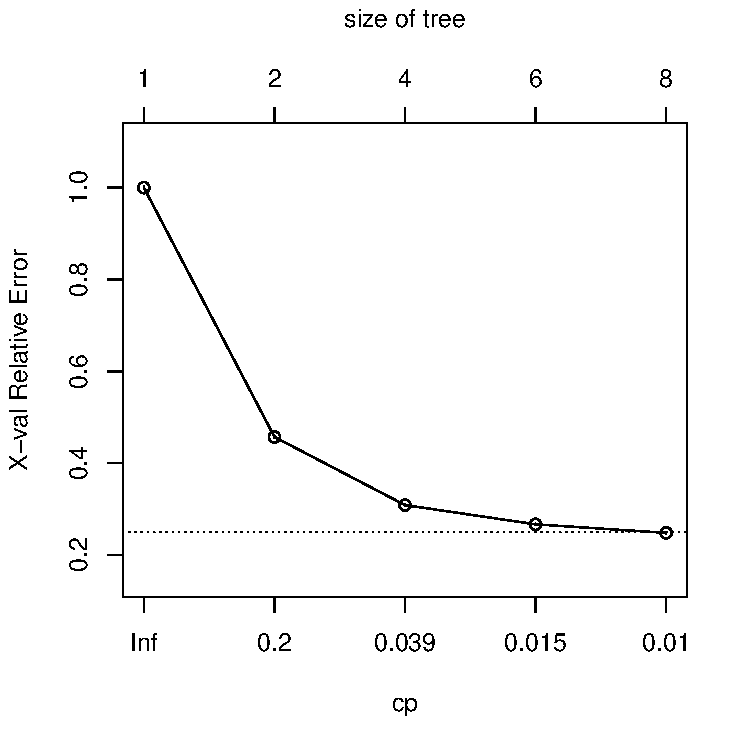
\includegraphics[width=0.7\linewidth]{../FinalResults/cptree}
	\caption{Grafico dell'andamento del parametro di complessità al crescere del numero di ramificazioni.}
	\label{fig:cptree}
\end{figure}
\begin{figure}
	\centering
	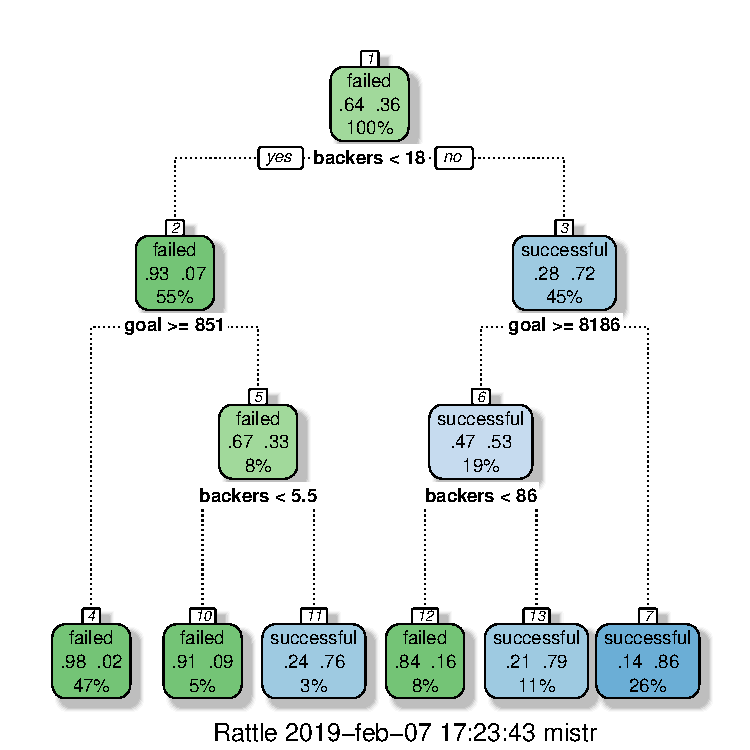
\includegraphics[width=0.7\linewidth]{../FinalResults/prunedtree}
	\caption{Albero risultante dalla potatura con valore del parametro cp pari a 0.015}
	\label{fig:prunedtree}
\end{figure}
\clearpage
\subsection{Na\"ive Bayes}
Il modello Na\"ive Bayes si basa sul Teorema di Bayes (si faccia riferimento alla Formula \ref{th:bayes}) e sull'assunzione che tutti gli attributi che descrivono le istanze sono condizionalmente indpendenti l'un l'altro.
\begin{equation}
\label{th:bayes}
P(h|D) = \frac{P(D|h) \cdot P(h)}{P(D)}
\end{equation}
Dove, nel nostro caso di interesse: h è un'ipotesi, D è l'insieme dei valori delle feature dell'istanza e l'operatore | indica la probabilità condizionata.\\
Il modello si basa quindi sullo stabilire l'ipotesi $h_{MAP}$, ovvero l'ipotesi massima a posteriori sfruttando la Formula \ref{for:hmap}, ovvero trovare l'ipotesi, tra le \textit{n} ipotesi disponibili, che massimizza il prodotto tra la probabilità a priori del verificarsi dell'ipotesi ($P(h_{i})$) e la produttoria tra i \textit{k} attributi delle relative verosimiglianze, rispetto all'ipotesi considerata, dell'assunzione da parte di tale attributo del valore che possiede il corrispettivo nell'istanza da classificare. 
Si noti che tale produttoria può essere calcolata grazie all'assunzione di indipendenza condizionale degli attributi.
Anche se non abbiamo formalmente mostrato tale ipotesi per il dataset utilizzato, vi sono casi in letteratura in cui tale modello ottiene delle buone performance in casi in cui gli attributi non sono condizionalmente indipendenti; di conseguenza abbiamo provato ad effettuare la predizione utilizzando questo modello.\\
\begin{equation}
	\label{for:hmap}
	h_{MAP} = argmax_{i = 0}^{n}\left(P(h_{i}) \cdot \prod_{j = 0}^{k}P(a_{j}|h_{i})\right)
\end{equation}
In termini pratici, riferendoci ad \emph{R}, il \texttt{trainset} è la matrice su cui calcolerà le varie probabilità a priori e le verosimiglianze per i vari attributi; il \texttt{trainset}, come al solito, saranno le istanze non etichettate da classificare.
L'implementazione del classificatore utilizzata è quella fornita nella libreria \texttt{e1071}, inoltre, per il suo utilizzo non sono state utilizzate impostazioni particolari.

In Figura \ref{fig:bayesperformance} sono rappresentati i boxplot per quanto riguarda le quattro misure di performance utilizzate, inoltre, nella Tabella \ref{tab:bayes_perf} sono rappresentate le relative medie e deviazioni standard; tali misure di performance sono state calcolate mediante un processo di 10-fold cross validation.
Valutando tali dati, notiamo che il classificatore Na\"ive Bayes è estremamente accurato ed ha alti valori sia di precisione che di recall, il che ci garantisce che quando viene predetto il fallimento di una campagna è altamemente probabile che fallisca, poiché sia il valore di recall che di precisione sono elevati.
Le curve ROC e le relativa AUC confermano ulteriormente quanto detto fin'ora; le singole ROC prodotte dai singoli passi del processo di 10-fold cross validation sono riportate in Figura \ref{fig:bayesROC}.

\begin{table}[h!]
	\caption{Tabella contenente la media e la deviazione standard rispetto alle misure di performance effettuate basandosi sull'esecuzione di una 10-fold cross validation sfruttando il modello Na\"ive Bayes.}
	
	\label{tab:bayes_perf}
	
	\centering
	\begin{tabular}{c|cc}
		Misura & Media & Deviazione standard \\
		\hline
		Accuratezza & 0.994 & 0.0005 \\
		Precisione & 0.995 &  0.0006\\
		Recall & 0.995 & 0.0004 \\
		F-measure & 0.995 & 0.0004 \\
	\end{tabular}
\end{table} 

\begin{figure}[h!]
	\centering
	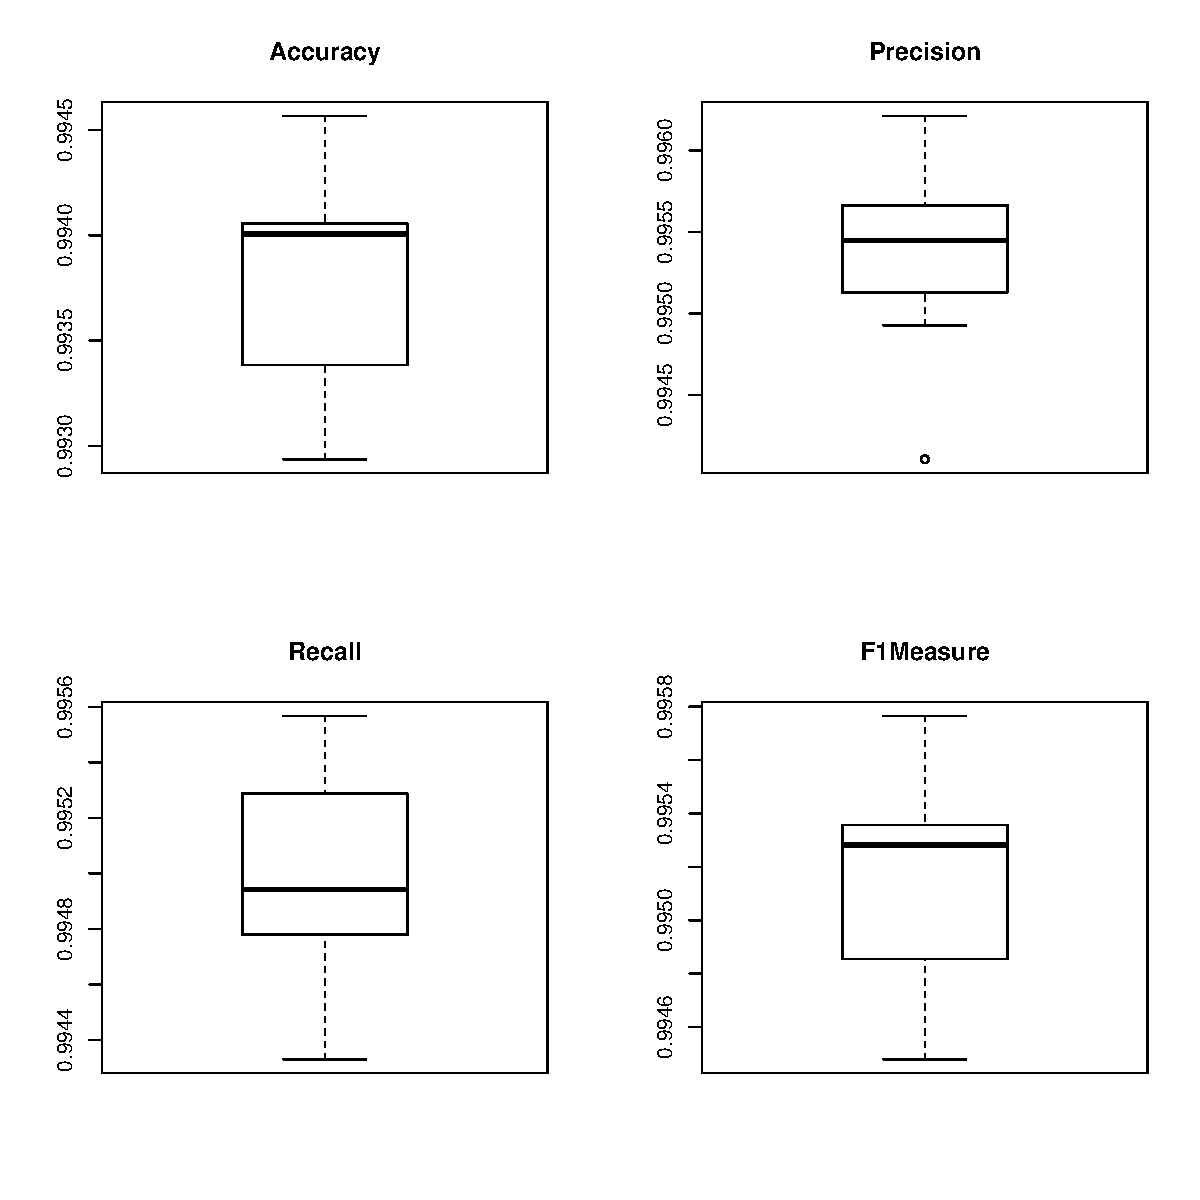
\includegraphics[width=0.7\linewidth]{../FinalResults/Bayes_performance}
	\caption{Boxplot relativi alle misure di performance del modello Na\"ive Bayes.}
	\label{fig:bayesperformance}
\end{figure}

\begin{figure}
	\centering
	\subfloat{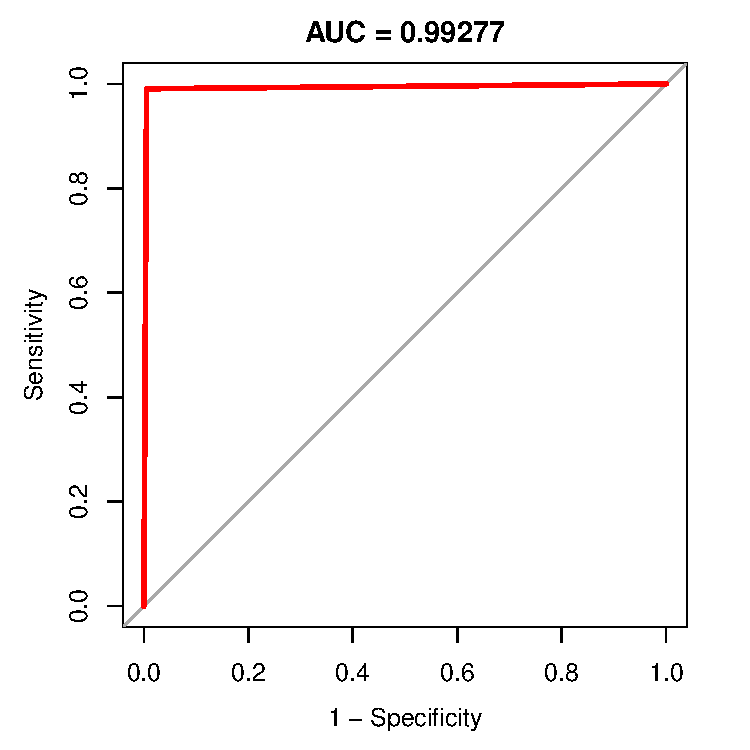
\includegraphics[width=0.3\linewidth]{../FinalResults/Images/bayes/auc_1.pdf}}\quad
	\subfloat{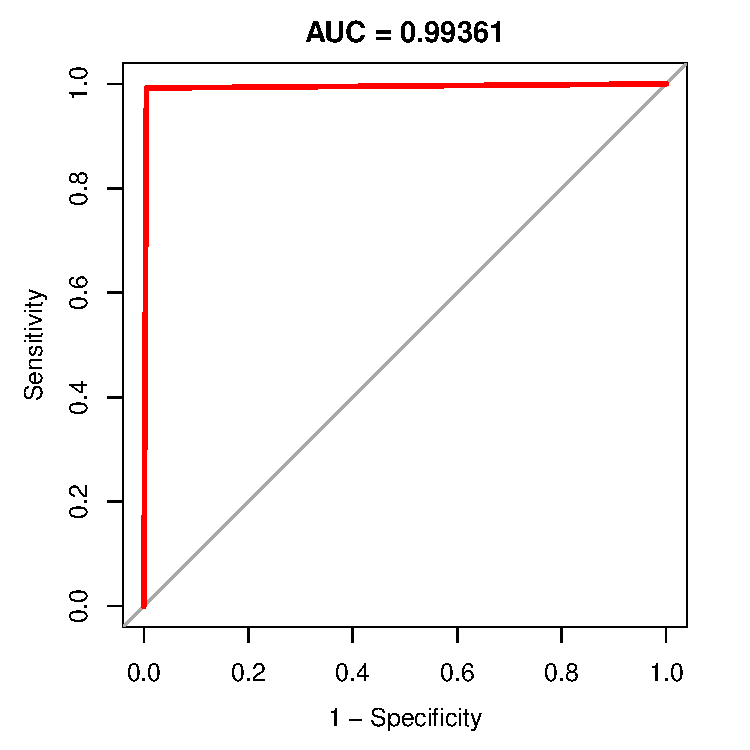
\includegraphics[width=0.3\linewidth]{../FinalResults/Images/bayes/auc_2.pdf}}\quad
	\subfloat{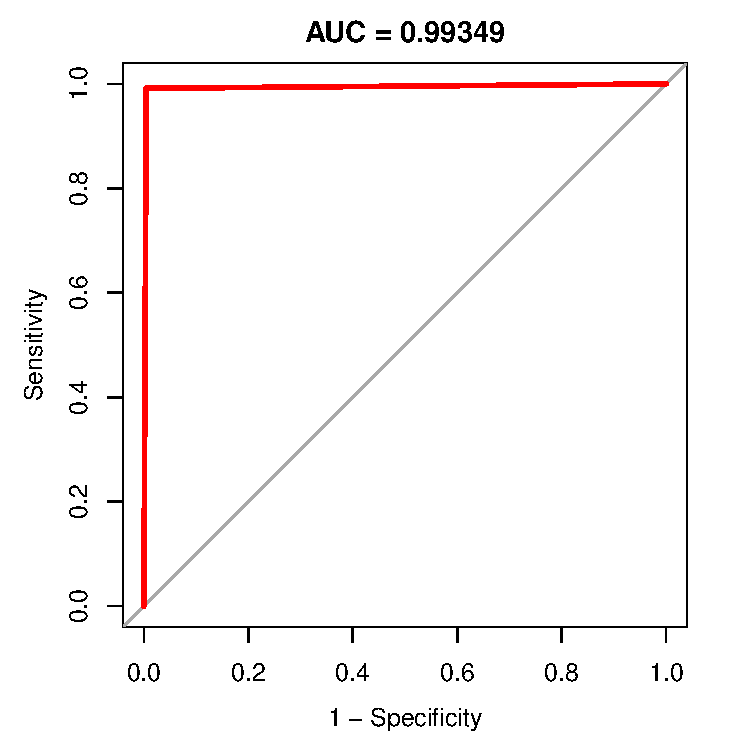
\includegraphics[width=0.3\linewidth]{../FinalResults/Images/bayes/auc_3.pdf}}\quad
	\subfloat{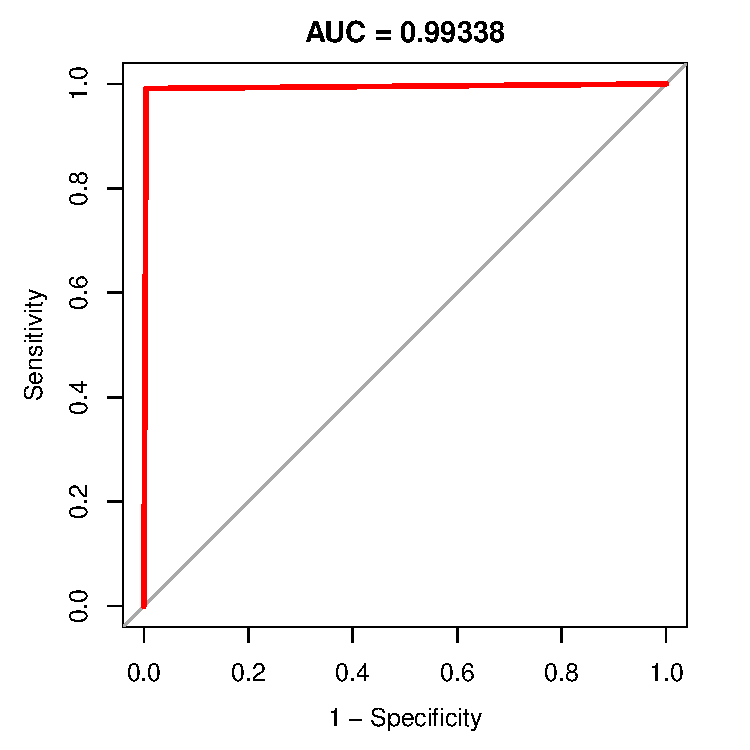
\includegraphics[width=0.3\linewidth]{../FinalResults/Images/bayes/auc_4.pdf}}\quad
	\subfloat{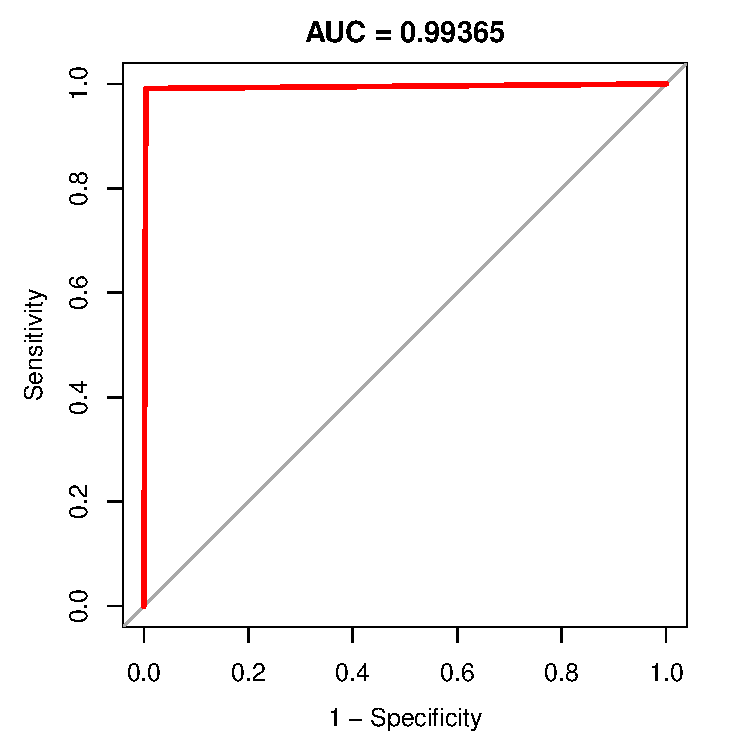
\includegraphics[width=0.3\linewidth]{../FinalResults/Images/bayes/auc_5.pdf}}\quad
	\subfloat{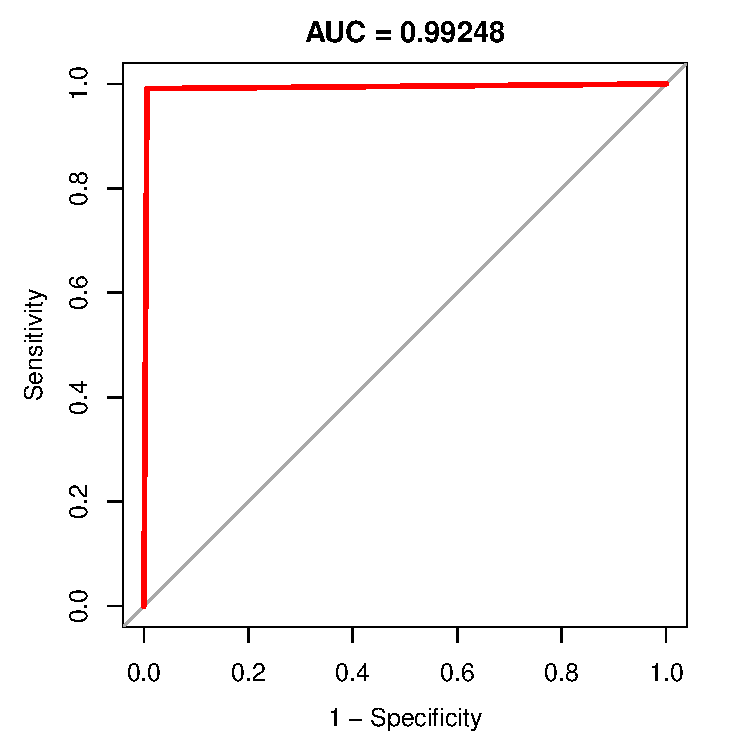
\includegraphics[width=0.3\linewidth]{../FinalResults/Images/bayes/auc_6.pdf}}\quad
	\subfloat{\includegraphics[width=0.3\linewidth]{../FinalResults/Images/bayes/auc_7.pdf}}\quad
	\subfloat{\includegraphics[width=0.3\linewidth]{../FinalResults/Images/bayes/auc_8.pdf}}\quad
	\subfloat{\includegraphics[width=0.3\linewidth]{../FinalResults/Images/bayes/auc_9.pdf}}\quad
	\subfloat{\includegraphics[width=0.3\linewidth]{../FinalResults/Images/bayes/auc_10.pdf}}\quad
	\caption{Curve ROC del modello Na\"ive Bayes per la 10-fold cross validation.}
	\label{fig:bayesROC}
\end{figure} 
\clearpage
\subsection{Support Vector Machine}
Le SVM (Support Vector Machine) sono algoritmi utilizzati sia per la classificazione binaria, ma non solo. 
Concettualmente si basano sul voler rappresentare le istanze in un iperspazio \textit{K}-dimensionale e ricercare un iperpiano separatore delle due classi, ottenendo così due semi-iperspazi in ciascuno dei quali sono presenti tutte e sole le istanze appartenenti ad una classe.
Risulta necessario sottolineare che non sempre è possibile suddividere l'insieme delle istanze mediante un iperpiano, perché le due classi potrebbero non essere linearmente separabili in un iperspazio \textit{K}-dimensionale.
Per ovviare a tale problema possono essere utilizzate sia delle trasformazioni geometriche in cui, generalmente, si aumentano le dimensioni dell'iperspazio (le quali portano a costi computazionali maggiori), oppure sfruttare i metodi Kernel che, brevemente, permettono di calcolare il risultato di tali trasformazioni rimanendo in \textit{K} dimensioni durante la computazione, renendo quindi il procedimento più efficiente.
Supponendo di avere le istanze nello spazio linearmente seprabili, poiché le classi lo sono nativamente o mediante l'utilizzo dei metodi Kernel, le SVM, di fatto, dovranno risolvere un problema di ottimizzazione: massimizzare il margine dell'iperpiano separatore.
Per far ciò, è quindi necessario identificare i vettori di supporto, ovvero l'insieme delle istanze che giacciono “vicino” al margine dell'iperpiano separatore.\\
Passando ad una trattazione più pratica rispetto al progetto, l'implementazione delle SVM utilizzata è quella fornita dalla libreria \texttt{e1071}; tale implementazione permette di specificare due parametri fondamentali:\begin{itemize}
	\item \texttt{kernel}, ovvero il metodo kernel utilizzato sia durante la fase di training che per la fase di \textit{testing}, alcune funzioni possibili sono \texttt{linear} o \texttt{sigmoid};
	\item \texttt{cost}, ovvero il costo di \textit{trade-off} tra la penalità derivante dalle variabili di slack e la larghezza del margine, ovvero più il valore del costo è basso più il margine sarà largo e potrebbe portare ad un maggiore errore nelle classificazioni, più è alto più il margine è strettoe meno errori di classificazione sono ammessi; si noti che potrebbero verificarsi casi di \textit{overfitting} causati da un'assegnazione del costo non ottimale. 
\end{itemize}
Poiché il tempo di training di tale implementazione delle SVM è molto oneroso in termini di tempo e dato che il dataset è composto da oltre 312 mila istanze, quindi il \textit{training set} da oltre 218 mila, si è deciso, di conseguenza, di effettuare il processo di training e di testing una sola volta, senza effettuare la 10-fold cross validation.
Abbiamo indagato le performance di due SVM differenti: la prima con un kernel lineare ed un costo pari ad 1, la seconda sempre con un kernel lineare ed un costo pari a 1000. 
La scelta di modificare solo il costo è stata dettata dalla decisione di valutare come cambiassero le performance mantenendo lo stesso metodo kernel, non sono stati testati altri metodi kernel poiché il tempo di training sarebbe stato troppo elevato (probabilmente ancora più elevato dei kernel lineari perché avrebbe implicato la computazione di funzioni più costose) ai fini del progetto, preferendo anche l'indagine del comportamento delle reti neurali; inoltre non si è voluta tentare un'operazione di \textit{automatic tuning} dei costi a causa dei tempi e neanche l'indagine del parametro \texttt{gamma} è stata effettuata poiché sono stati utilizzati solo kernel lineari.

Valutando complessivamente le performance, i cui dati sono riportati in Tabella \ref{tab:svm_perf} e \ref{tab:svm1000_perf} e le cui relative ROC sono rappresentate in Figura \ref{fig:svmperformance} e \ref{fig:svm1000performance}, possiamo concludere che il modello il cui costo è pari ad 1 porta ad una minore precisione, come ci si poteva attendere dato il ruolo del costo, inoltre anche la differenza nella precisione è figlia della stessa causa.
Risulta particolare che il valore di default rimanga praticamente lo stesso (un \textit{delta} per a 0.009), questo significa che ambo le SVM classificano correttamente le campagne veramente fallimentari allo stesso modo ma nel farlo la prima produce un numero maggiore di falsi positivi (ovvero campagne predette come fallimentari, ma che se avviate avrebbero successo). 
Inoltre, andando ad analizzare il numero di vettori di supporto utilizzati per lo stabilimento del margine, si nota che la SVM il cui costo è 1 ha utilizzato ne ha utilizzati più di 81 mila, al contempo la seconda ne ha utilizzati circa 61 mila; questa differenza è ancora una volta data dal fatto che un costo più alto provoca l'utilizzo di un margine più ristretto e di conseguenza un utilizzo di un numero minore di vettori di supporto.
Concludendo, anche le ROC e relative AUC sono molto simili tra loro il che implica che la sensitività, come mostrato dai dati riportati nelle tabelle sopra citata, e specificità dei due modelli sono rispettivamente molto vicine tra loro.

\begin{table}
	\caption{Tabella contenente le performance per quanto riguarda il modello SVM con il costo pari a 1 ed il kernel lineare.}
	
	\label{tab:svm_perf}
	
	\centering
	\begin{tabular}{c|c}
		Misura & valore \\
		\hline
		Accuratezza & 0.884 \\
		Precisione & 0.873 \\
		Recall & 0.958 \\
		F-measure & 0.913 \\
	\end{tabular}
\end{table}

\begin{table}
	\caption{Tabella contenente le performance per quanto riguarda il modello SVM con il costo pari a 1000 ed il kernel lineare.}
	
	\label{tab:svm1000_perf}
	
	\centering
	\begin{tabular}{c|c}
		Misura & valore \\
		\hline
		Accuratezza & 0.908 \\
		Precisione & 0.910 \\
		Recall &  0.949\\
		F-measure & 0.929 \\
	\end{tabular}
\end{table}

\begin{figure}
	\centering
	\includegraphics[width=0.7\linewidth]{../FinalResults/Images/svm/auc.pdf}
	\caption{Boxplot relativi alle misure di performance del modello SVM con costo pari a 1.}
	\label{fig:svmperformance}
\end{figure}

\begin{figure}[h]
	\centering
	\includegraphics[width=0.7\linewidth]{../FinalResults/Images/svm1000/auc.pdf}
	\caption{Boxplot relativi alle misure di performance del modello SVM con costo pari a 1000.}
	\label{fig:svm1000performance}
\end{figure}
\clearpage
\subsection{Reti neurali}
Le reti neurali sono un modello che si è rivelato non performare come sperato per il nostro caso di studio. L'assenza di conoscenza pregressa circa una possibile topologia della rete e l'abbondanza di parametri che influiscono sulla corretta convergenza dell'algoritmo di apprendimento ha portato alla impossibilità di produrre un modello funzionante. Sono stati effettuati numerosi test per trovare la corretta combinazione di parametri, modificando il numero di neuroni nascosti, il numero massimo di iterazioni del processo di learnig e il valore di learning rate della rete; seppur alcuni test su scala ridotta abbiano prodotto un modello funzionante e dalle performance accettabili (riportate in Tabella \ref{tab:nnperformance}), ogni tentativo di training della rete sull'intero dataset ha portato alla non convergenza del processo. Abbiamo quindi deciso di non includere questo modello nella nostra analisi, in quanto non è stato possibile replicare i risultati ottenuti su scala ridotta su tutto il dataset. Altri fattori che hanno contribuito all'esclusione di questo modello sono il lungo tempo di training della rete al crescere del numero di neuroni e di sample in input.

\begin{table}
	\caption{Tabella che riporta i valori delle misure di performance sulla rete trainata su 1000 sample del dataset.}
	\label{tab:nnperformance}
	\centering
	\begin{tabular}{c|c}
		Misura & valore \\
		\hline
		Accuracy & 0.8953  \\ 
		Precision & 0.9808  \\
		Recall & 0.8521  \\
		F1Measure & 0.9119  \\
	\end{tabular}
\end{table}

\subsection{Confronto tra modelli}
I modelli presentati nelle sezioni precedenti hanno mostrato pregi e difetti, che saranno ora velocemente riassunti.
Gli alberi decisionali hanno mostrato un utilizzo limitato delle feature del dataset, limitandosi a sfruttare solo due delle 7 feature disponibili. Ciò porta a performance non ottimali del modello durante la classificazione di nuovi sample. A loro favore, il training e la classificazioni risultano molto veloci.\\
Il modello Na\"ive Bayes ha prodotto performance ottimali, risultando rapido sia nella fase di addestramento che nella fase di classificazione. L'unica mancanza riscontrata è l'assenza di parametri per la personalizzazione del processo di learning, che non si è però tramutata in una problematica in quanto i risultati prodotti si sono rivelati più che soddisfacente.\\
Le SVM hanno mostrato un tempo di training e di classificazione molto elevato a confronto dei modelli precedentemente discussi, fornendo però prestazioni leggermente superiori agli alberi di decisioni ottenuti.\\
Le reti neurali hanno mostrato tempi di training sproporzionatamente elevati rispetto alle altre tecniche indagate, non portando ad un risultato utilizzabile per la classificazione.\\
La Figura \ref{fig:mixed2} mostrano le curve ROC dei modelli ottenuti a confronto. Il modello che spicca su tutti è il Na\"ive Bayes, che risulta  avere una AUC corrispondente alla curva superiore a $0.99$; alberi di decisione e SVM seguono “a parimerito”, mentre infine troviamo l'albero di decisione privo dell'attributo backer.
Le curve ROC rappresetate sono le curve inerenti alla decima iterazione del processo di 10-fold cross validation, mentre per le SVM sono rappresentate le due curve ROC analizzate in precedenza.
Rappresentare una sola ROC per curva non è limitativo poiché come mostrato in precedenza hanno un comportamento molto analogo in tutte e 10 le iterazioni, l'unico caso differente è la baseline poiché da come viene partizionato il dataset può avere casi “fortunati” in cui predice molto bene, ma come visto sono casi particolare e la sua tendenza è comportarsi in un modo analogo alla curva mostrata in figura.
\begin{figure}
	\centering
	\includegraphics[width=0.9\linewidth]{../FinalResults/Images/Mixed2}
	\caption{Curve ROC dei modelli presentati nella relazione, sono state riportate le ROC della decima iterazione del processo di 10-fold cross validation di ogni modello analizzato e le ROC delle SVM.}
	\label{fig:mixed2}
\end{figure}
